
%	Event selection

\section{Event selection}\label{Section_Selection}
\Headerfooter{Event selection}
\vs\hs
In this study, we search for NCQE events that consist of prompt signals from de-excitation gamma-rays and delayed signals from neutrons.
We select events where the visible energy of the prompt signal ($E_{{\rm vis}}$) is between 7.49~MeV and 29.49~MeV because most NCQE events are in the $E_{{\rm vis}}$ region (see Figure~\ref{FTFP_BERT_HP_Figure08_Poisson}).
In each candidate event, delayed signals within 535 $\mu$s from the prompt signal are searched.
The event reconstruction and neutron tagging method follow the DSNB search in SK-Gd phase~\cite{2023Harada,2022Harada}.
%Details of the neutron tagging method are summarized in Section~6 of Ref.~\cite{2023HaradaPhD}.\\
Details of the neutron tagging method are summarized in Section~\ref{Subsubsec_Ndelayed}.\\
\hs
The data sample includes not only NCQE events but also other events such as atmospheric neutrino NC non-QE events, atmospheric neutrino charged-current (CC) events, spallation events (see Section~\ref{Subsubsec_sim_spa}), reactor neutrino events (see Section~\ref{Subsubsec_sim_reactor}), and accidental coincidence events.
Most of atmospheric neutrino NC non-QE events ($\sim$90.4\% of NC non-QE events after applying all event selections) are events with single meson, as shown in Figure~\ref{Selection_NC_single_meson}.
Schematic view of atmospheric neutrino CC events is shown in Figure~\ref{Selection_CC_nue_CC_numu}.
Muon neutrino CC events become backgrounds when the emitted muon is invisible (below Cherenkov threshold (see Section~\ref{subsec_detect_princi})).
Accidental coincidence events are mainly pairs of a spallation event without neutrons and a neutron misidentification event.
Most of these events can be removed by applying various event reductions.
However, some events remain even after applying all event reductions.
To determine the number of NCQE events, it is necessary to estimate the number of all those events.
The methods of event reduction and event estimation are described below.\\
\hs
This study uses 552.2~days of data with 0.011\% gadolinium-loaded water from August 2020 to June 2022.
This data set is the same as the one used for the SK-Gd DSNB search~\cite{2023Harada}.

\begin{figure}[h]
	\centering
	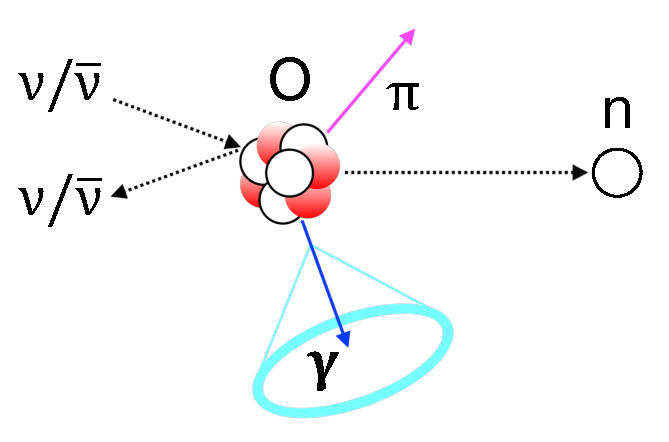
\includegraphics[width=6cm]{Figures/Selection/NC_single_meson}
	\caption[Schematic view of an atmospheric neutrino NC event with single meson]{
	Schematic view of an atmospheric neutrino NC event with single meson.
	}\label{Selection_NC_single_meson}
\end{figure}

\begin{figure}[h]
	\centering
	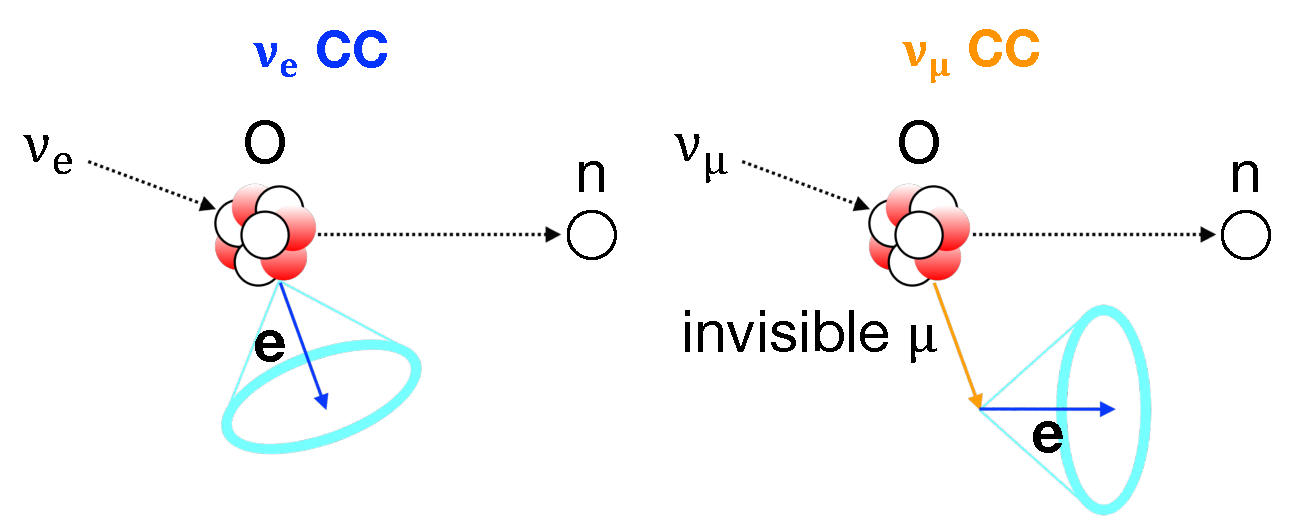
\includegraphics[width=12cm]{Figures/Selection/CC_nue_CC_numu}
	\caption[Schematic view of atmospheric neutrino CC events]{
	Schematic view of atmospheric neutrino CC events.
	}\label{Selection_CC_nue_CC_numu}
\end{figure}





\subsection{First reduction: Pre-cut}
\subsubsection{Non-SHE-triggered event and noise event cut}
\vs\hs
First, when a run satisfies the following conditions, events in the run are not used.
\begin{itemize}
	\item Run time is shorter than 5~minutes
	\item Run started less than 15~minutes after the high-voltage was recovered
	\item Any hardware problem is reported
	\item Event distribution is unusual due to detector problems
\end{itemize}
\hs
Moreover, the following events are removed.
\begin{itemize}
	\item Calibration trigger events
	\item Periodic trigger events
	\item T2K beam trigger events
	\item Pedestal events
\end{itemize}
\hs
In addition, the condition $N(Q < 0.5\,{\rm p.e.})/N_{\rm total} < 0.55$ is required to remove the events triggered by PMT noise hits, where $N(Q < 0.5\,{\rm p.e.})$ is the number of hits with a charge smaller than $0.5\,{\rm p.e.}$ and $N_{\rm total}$ is the total number of hits.

\subsubsection{Cosmic ray muon-induced event cut}
\vs\hs
Cosmic ray muons come to the SK at $\sim$2~Hz, and most of these muons issue the OD trigger.
To remove events induced by cosmic ray muons, events that the OD trigger is issued are not used.
Moreover, some muons decay into electrons with a life time of 2.2~$\mu$s, leaving hits inside the ID without an OD trigger.
To remove events induced by these electrons, events within 50~$\mu$s from preceding cosmic ray muons are not used.
Spallation events caused by cosmic ray muons will be described later.

\subsubsection{Fiducial volume cut}
\vs\hs
Radioactive backgrounds are concentrated near the detector wall.
Therefore, events within 2~m away from the ID wall are removed.

\subsubsection{Fit quality cut}
\vs\hs
To remove poorly reconstructed events, events that the vertex reconstruction goodness ($g_{\rm vtx}$) is less than 0.5 are removed.
Details of $g_{\rm vtx}$ are summarized in Section~\ref{Subsec_vertex_rec}.

\subsubsection{Trigger requirement}
\vs\hs
To search delayed signals within 535~$\mu$s from the prompt signal, not only the SHE trigger but also the AFT trigger must be issued.
However, since the AFT trigger rate was limited to once every 21~ms until the middle of SK-VI, some events did not issue the AFT trigger.
Therefore, in MC, the number of events is scaled by using the AFT trigger efficiency $\varepsilon_{\rm AFT}$ defined as
\begin{eqnarray}
	\varepsilon_{\rm AFT} = {N_{\rm AFT} \over N_{\rm SHE}},
\end{eqnarray}
where $N_{\rm AFT}$ is the number of AFT-triggered events and $N_{\rm SHE}$ is the number of SHE-triggered events.
$\varepsilon_{\rm AFT}$ is summarized in Table~\ref{tab:AFT}.

\begin{table}[h]
	\centering
	\caption[AFT trigger efficiency considering the whole period of SK-VI]{
	AFT trigger efficiency considering the whole period of SK-VI.
	}\label{tab:AFT}
	\vs
	\begin{tabular}{cc} \hline \hline
		$E_{\rm vis}$ & $\varepsilon_{\rm AFT}$ \\
		(MeV)         &                         \\ \hline
		7.49--9.49    & 85.3\%                  \\
		9.49--11.49   & 80.4\%                  \\
		11.49--13.49  & 74.3\%                  \\
		13.49--15.49  & 70.0\%                  \\
		15.49--17.49  & 67.9\%                  \\
		17.49--19.49  & 63.4\%                  \\
		19.49--21.49  & 89.7\%                  \\
		21.49--23.49  & 90.0\%                  \\
		23.49--25.49  & 90.0\%                  \\
		25.49--27.49  & 100.0\%                 \\
		27.49--29.49  & 90.5\%                  \\ \hline \hline
	\end{tabular}
\end{table}





\subsection{Second reduction: Spallation cut}
\vs\hs
Here, the spallation events, which are major backgrounds in the energy range from a few MeV to tens of MeV, are removed.
As described in Section~\ref{Subsubsec_sim_spa}, some radioactive isotopes produced by cosmic-ray muon spallation of oxygen nuclei mimic the IBD and NCQE events.
The spallation cut consists of five components, and these components are described in Section~\ref{Sec_1ms} to Section~\ref{Sec_box}.

\subsubsection{1~ms cut}\label{Sec_1ms}
\vs\hs
Gamma-rays and neutrons are emitted by hadronic nuclear interactions caused by nucleons and mesons with hundreds of MeV generated by muon spallation.
In some cases, the gamma-rays can issue the SHE trigger, and the neutrons can be detected as delayed signals.
To remove these events, events within 1~ms from preceding cosmic ray muons are not used.

\subsubsection{Multiple spallation cut}
\vs\hs
Energetic cosmic ray muons may produce multiple radioactive isotopes.
When a spallation event issues the SHE trigger, other spallation events may be observed close to the event both in time and space.
To remove the SHE-triggered events, low energy events with a $E_{\rm vis}$ of 5.49--24.49~MeV within $\pm$60~s from the SHE-triggered event are used.
First, selection criteria of the solar neutrino analysis~\cite{2016Abe} are applied to all low energy events.
Then, the distance from the SHE-triggered event to each low energy event is calculated.
If there is one low energy event with a distance of less than 4.0~m, the SHE-triggered event is removed (see Figure~\ref{Selection_multiple_spa}).

\begin{figure}[h]
	\centering
	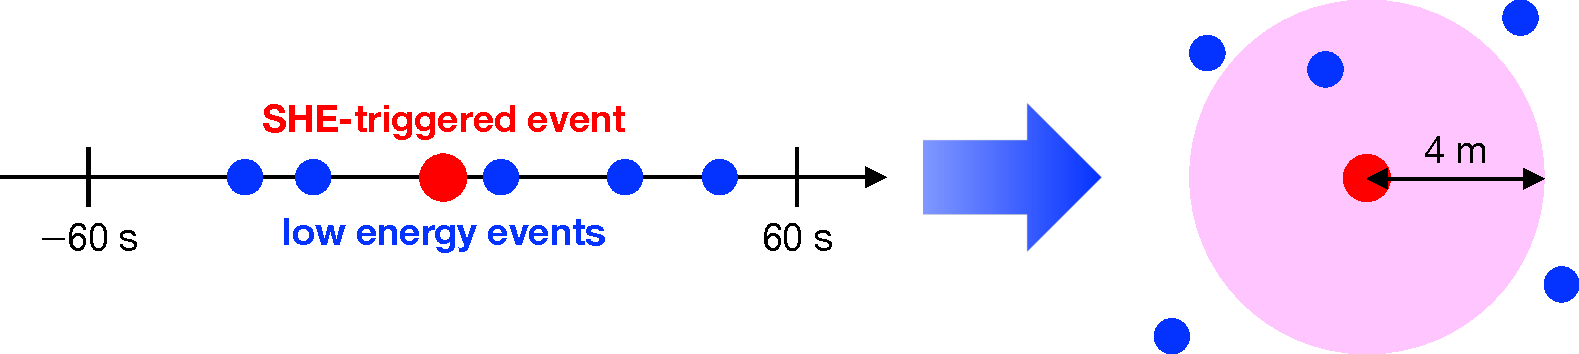
\includegraphics[width=12cm]{Figures/Selection/multiple_spa}
	\caption[Schematic view of multiple spallation cut]{
	Schematic view of multiple spallation cut.
	In this case, the SHE-triggered event is removed.
	}\label{Selection_multiple_spa}
\end{figure}

\subsubsection{Neutron cloud cut}
\vs\hs
Muon spallation produces many particles, including neutrons.
These neutrons are captured on Gd, and generate neutron event clusters, named neutron cloud, near the spallation point.
To remove spallation events, the information of neutron cloud is used.
First, the following selection criteria are applied to neutron events after muon spallation.
\begin{itemize}
	\item $N_{200} \geq 25$
	\item Timing is within [35, 535]~$\mu$s from the muon spallation
	\item $g_{\rm vtx} > 0.4$ and $g_{\rm dir} < 0.4$
	\item Distance from the muon track is within 5~m
\end{itemize}
Here, $N_{200}$ is the number of hits in a TOF-subtracted 200~ns time window and $g_{\rm dir}$ is the direction reconstruction goodness.
Details of $g_{\rm dir}$ are summarized in Section~\ref{Subsec_direction_rec}.
These selection criteria are based on the measurement of cosmogenic neutron yield in SK-Gd~\cite{2023Shinoki}.
If the number of neutron events that satisfied the above selection criteria ($N_{\rm cloud}$) is greater or equal to 2, the muon is considered to have a neutron cloud.
Then, SHE-triggered events are removed based on cut criteria summarized in Table~\ref{tab:ncloud}.
In Table~\ref{tab:ncloud}, $\Delta T$ is the time difference between the muon and SHE-triggered event and $\Delta l$ ($= \Delta_{x}^{2} + \Delta_{y}^{2} + \Delta_{z}^{2}$) is the distance ilustrated in Figure~\ref{def_ncloud}.

\begin{table}[h]
	\centering
	\caption[Cut criteria of neutron cloud cut]{
	Cut criteria of neutron cloud cut~\cite{2023HaradaPhD}.
	The cut criteria are based on the SK DSNB analysis~\cite{2021Abe}.
	}\label{tab:ncloud}
	\vs
	\begin{tabular}{ccr} \hline \hline
		                              & Time [s]         & Spatial [cm]                                                                           \\ \hline
		$N_{\rm cloud} \geq 2$        & $\Delta T < 0.1$ & $\Delta l < 1,200$                                                                     \\
		$N_{\rm cloud} \geq 2$        & $\Delta T < 1$   & $\Delta l < 800$                                                                       \\
		$N_{\rm cloud} = 2$           & $\Delta T < 30$  & $(\Delta_{x}^{2} + \Delta_{y}^{2})/200^{2} + \Delta_{z}^{2}/400^{2} > 1.2$             \\
		$N_{\rm cloud} = 3$           & $\Delta T < 60$  & $(\Delta_{x}^{2} + \Delta_{y}^{2})/(6 \times 10^{4}) + \Delta_{z}^{2}/500^{2} > 1.2$   \\
		$4 \leq N_{\rm cloud} \leq 5$ & $\Delta T < 60$  & $(\Delta_{x}^{2} + \Delta_{y}^{2})/(1.2 \times 10^{5}) + \Delta_{z}^{2}/550^{2} > 1.2$ \\
		$6 \leq N_{\rm cloud} \leq 9$ & $\Delta T < 60$  & $(\Delta_{x}^{2} + \Delta_{y}^{2})/(2 \times 10^{5}) + \Delta_{z}^{2}/650^{2} > 1.2$   \\
		$N_{\rm cloud} \geq 10$       & $\Delta T < 60$  & $(\Delta_{x}^{2} + \Delta_{y}^{2})/500^{2} + \Delta_{z}^{2}/700^{2} > 1.2$             \\ \hline \hline
	\end{tabular}
\end{table}

\begin{figure}[h]
	\centering
	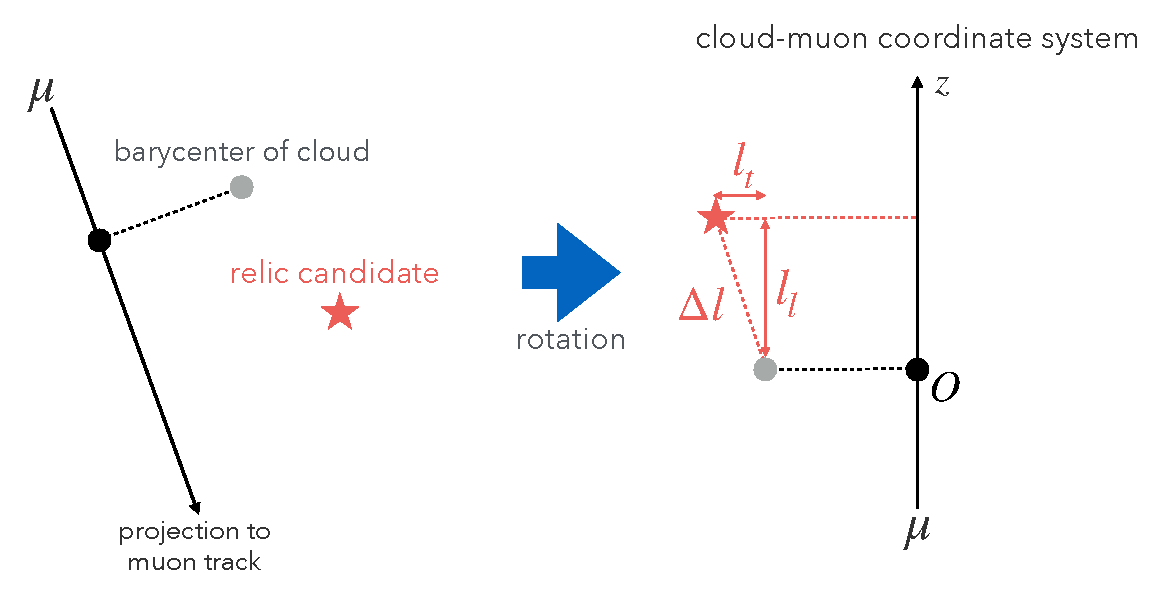
\includegraphics[width=12cm]{Figures/Selection/def_ncloud}
	\caption[Definition of the variables used in the neutron cloud cut]{
	Definition of the variables used in the neutron cloud cut~\cite{2023HaradaPhD}.
	}\label{def_ncloud}
\end{figure}

\subsubsection{Spallation likelihood cut}
\vs\hs
To further remove spallation events, the spallation likelihood is used.
The spallation likelihood $\mathcal{L}_{\rm spall}$ is defined as
\begin{eqnarray}
	\mathcal{L}_{\rm spall} = {\rm log}\prod_{i} \Bigg\{{{\rm PDF}^{i}_{\rm spall}(x) \over {\rm PDF}^{i}_{\rm random}(x)}\Bigg\},
\end{eqnarray}
where ${\rm PDF}^{i}_{\rm spall}$ is the probability density function (PDF) of the muon spallation sample, ${\rm PDF}^{i}_{\rm random}$ is the PDF of the random sample, $i$ is the $i$-th valiable used in the calculation, and $x$ is the value of the $i$-th variable.
Definition of the muon spallation sample and the random sample is summarized in Figure~\ref{Selection_pre_post}~\cite{2023HaradaPhD}.

\begin{figure}[tbp]
	\centering
	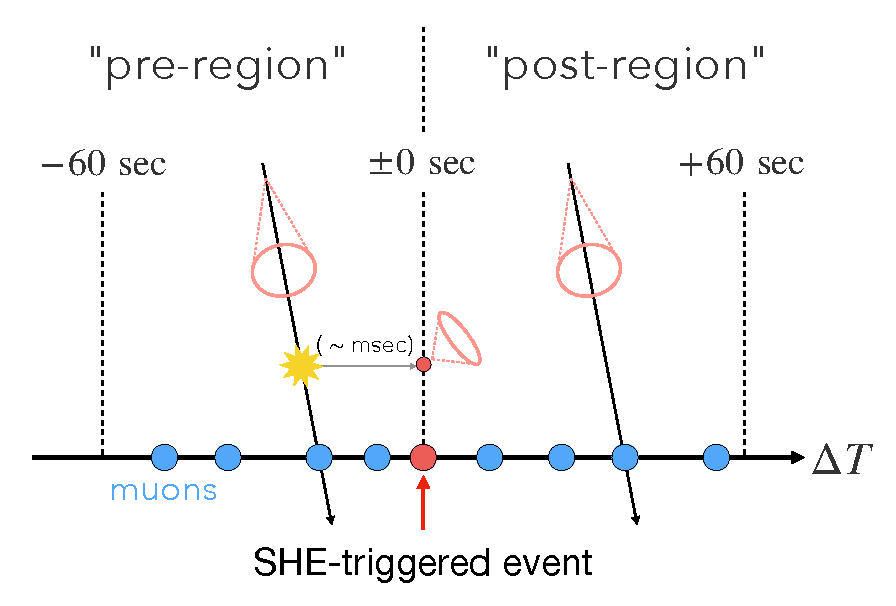
\includegraphics[width=10cm]{Figures/Selection/pre_post}
	\caption[Definition of the muon spallation sample and the random sample]{
	Definition of the muon spallation sample and the random sample~\cite{2023HaradaPhD}.
	Pre-region includes both muon spallation samples (muon events correlated with the SHE-triggered event) and random samples (muon events uncorrelated with the SHE-triggered event), while post-region includes only random samples.
	}\label{Selection_pre_post}
\end{figure}

\hs
There are five variables used in the calculation as follows.
\begin{itemize}
	\item $dt$: Time difference between the muon and SHE-triggered event.
	For spallation events, this variable should reflect lifetimes of the produced radioactive isotopes.
	\item $l_{t}$: Transverse distance from the muon track to SHE-triggered event.
	For spallation events, this variable should be within a few meters.
	\item $l_{l}$: Longitudinal distance from the maximum energy deposition point on the muon track to SHE-triggered event.
	The maximum energy deposition point is correlated to the spallation point, and this variable should be within a few meters for spallation events. 
	\item $Q_{\mu}$: Total charge deposited by the muon in the ID.
	$Q_{\mu}$ of spallation events should be larger than $Q_{\mu}$ expected from the minimum ionization.
	\item $Q_{\rm res}$: Difference between $Q_{\mu}$ and charge expected from the minimum ionization, defined as
	\begin{eqnarray}
		Q_{\rm res} = Q_{\mu} - Q_{\rm MI} \times L,
	\end{eqnarray}
	where $Q_{\rm MI}$ is the number of photoelectrons per centimeter expected from the minimum ionization and $L$ is the muon track length.
	For multiple muons, $L$ is the sum of muon track lengths.
	$Q_{\rm res}$ indicates the probability that a muon will cause nuclear spallation.
\end{itemize}
Figure~\ref{def_likelihood} shows the definition of $l_{t}$ and $l_{l}$ used in the spallation likelihood cut.\\
\hs
${\rm PDF}^{i}_{\rm spall}$ and ${\rm PDF}^{i}_{\rm random}$ are made for four muon types, single-through going, stopping, multiple, and misfit muons, categorized at a muon reconstruction algorithm (Muboy)~\cite{1997ConnerPhD,2004DesaiPhD,2023HaradaPhD}.
Figure~\ref{muon_type} shows the schematic view of a single-through going muon, a stopping muon, and multiple muons.
In Muboy, when the number of PMT hits is less than a certain threshold, the muon is categorized as a misfit muon.
For misfit muons, only PDFs for $dt$ are used to calculate $\mathcal{L}_{\rm spall}$ because the number of PMT hits is small and other variables are unreliable.
For single-through going, stopping, and multiple muons, PDFs for $l_{l}$, $Q_{\mu}$, and $Q_{\rm res}$ used to calculate $\mathcal{L}_{\rm spall}$ change depending on the values of $dt$ (0--0.05~s, 0.05--0.5~s, 0.5--60~s) and $l_{t}$ (0--300~cm, 300--1,000~cm, 1,000--5,000~cm).
Figure~\ref{PDF} shows the PDFs of the muon spallation sample and the random sample for single-through going muons ($dt$: 0--0.05~s, $l_{t}$: 0--300~cm).
These PDFs are clearly different between muon spallation samples and random samples.
Details about how to make PDFs are summarized in Ref.~\cite{2023HaradaPhD}.\\
\hs
$\mathcal{L}_{\rm spall}$ is calculated for all muons in time region from $-$60~s to 60~s with the SHE-triggered event as 0~s.
If just one value of $\mathcal{L}_{\rm spall}$ exceeds the cut criterion, the SHE-triggered event is removed.
Cut criteria of $\mathcal{L}_{\rm spall}$ depend on muon type and $E_{\rm vis}$.
For single-through going and multiple muons, the cut criteria change depending on $dt$ and $l_{t}$.
Cut criteria of spallation likelihood cut for each muon type are summarized in Table~\ref{tab:cut_single} to Table~\ref{tab:cut_misfit}.
Figure~\ref{L_spall} shows the $\mathcal{L}_{\rm spall}$ distributions when $E_{\rm vis}$ is between 7.49~MeV and 9.49~MeV.

\begin{figure}[tbp]
	\centering
	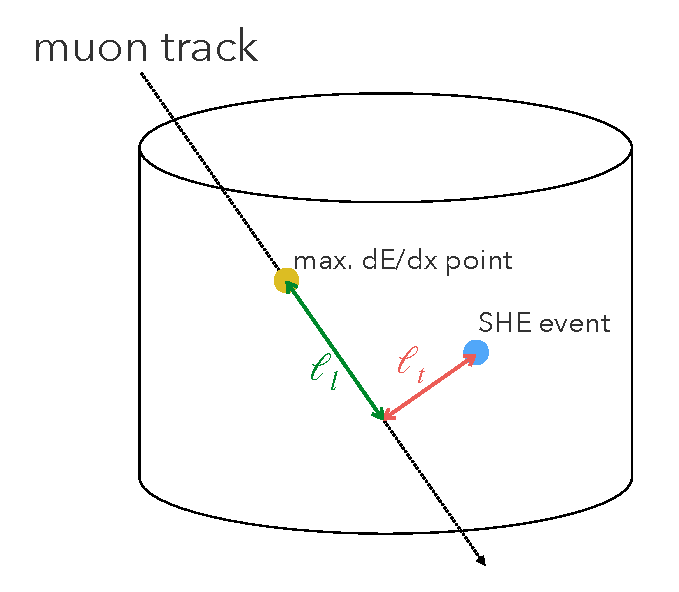
\includegraphics[width=8cm]{Figures/Selection/def_likelihood}
	\caption[Definition of $l_{t}$ and $l_{l}$ used in the spallation likelihood cut]{
	Definition of $l_{t}$ and $l_{l}$ used in the spallation likelihood cut~\cite{2023HaradaPhD}.
	}\label{def_likelihood}
\end{figure}

\begin{figure}[tbp]
	\centering
	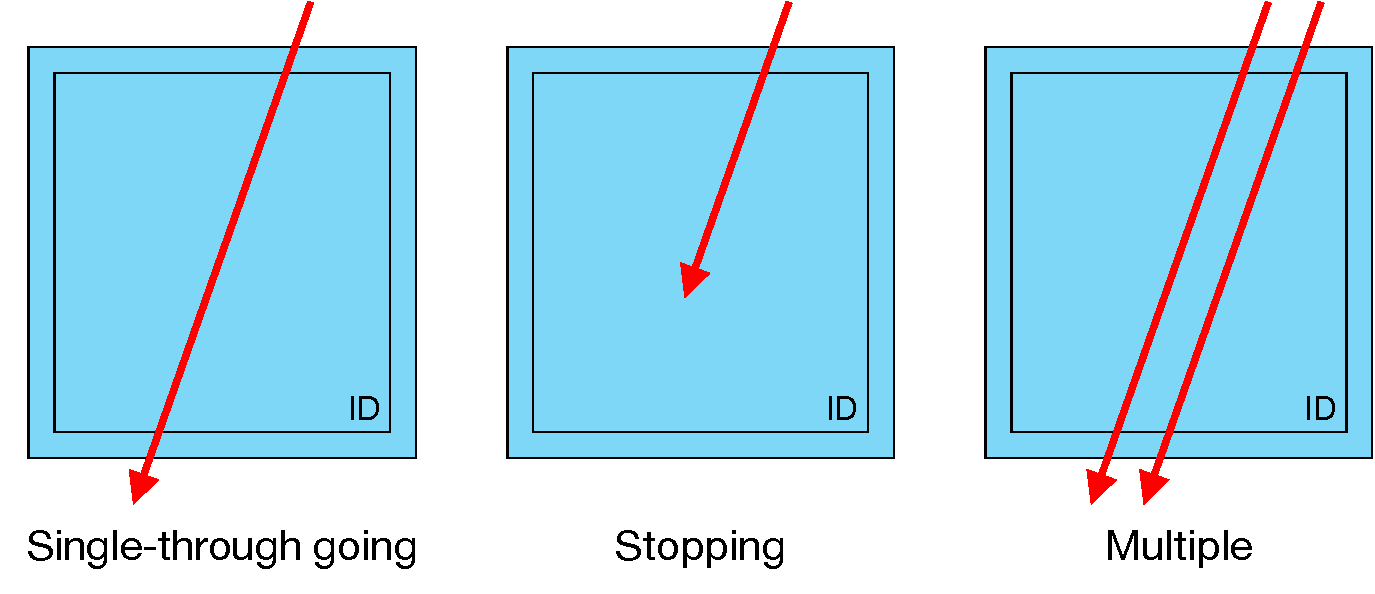
\includegraphics[width=12cm]{Figures/Selection/muon_type}
	\caption[Schematic view of a single-through going muon, a stopping muon, and multiple muons]{
	Schematic view of a single-through going muon, a stopping muon, and multiple muons.
	}\label{muon_type}
\end{figure}

\begin{figure}[tbp]
	\centering
	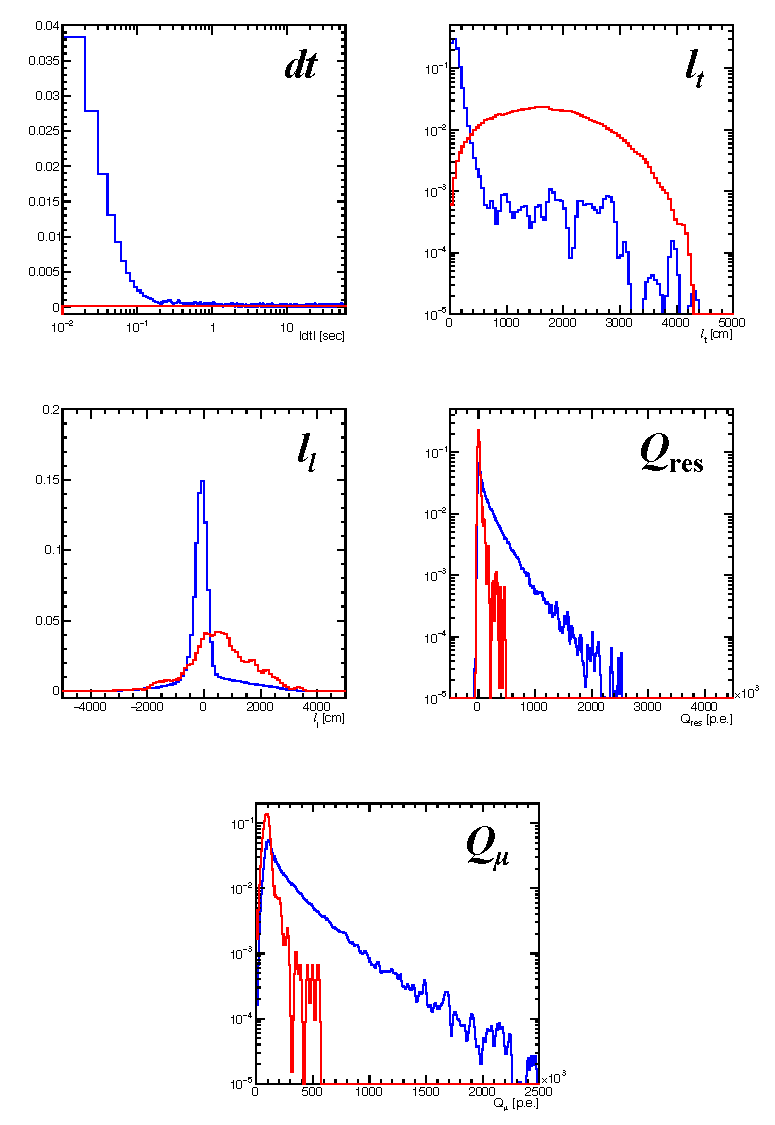
\includegraphics[width=14cm]{Figures/Selection/PDF}
	\caption[PDFs of the muon spallation sample and the random sample for single-through going muons ($dt$: 0--0.05~s, $l_{t}$: 0--300~cm)]{
	PDFs of the muon spallation sample (blue line) and the random sample (red line) for single-through going muons ($dt$: 0--0.05~s, $l_{t}$: 0--300~cm)~\cite{2023HaradaPhD}.
	}\label{PDF}
\end{figure}

\begin{table}[p]
	\centering
	\caption[Cut criteria of spallation likelihood cut for single-through going muons]{
	Cut criteria of spallation likelihood cut for single-through going muons.
	$\mathcal{L}_{\rm spall}$ distributions are shown in Figure~\ref{L_spall}.
	}\label{tab:cut_single}
	\vs
	\begin{tabular}{ccccc} \hline \hline
		$E_{\rm vis}$ (MeV)      & 7.49--9.49                        & 9.49--11.49                      & 11.49--13.49                     & 13.49--15.49                     \\ \hline
		$dt$: 0--0.05~s          & $\mathcal{L}_{\rm spall} > 15.5$  & $\mathcal{L}_{\rm spall} > 18$   & $\mathcal{L}_{\rm spall} > 17.5$ & $\mathcal{L}_{\rm spall} > 17.5$ \\
		$dt$: 0.05--0.5~s        & $\mathcal{L}_{\rm spall} > 17$    & $\mathcal{L}_{\rm spall} > 18$   & $\mathcal{L}_{\rm spall} > 18.5$ & $\mathcal{L}_{\rm spall} > 18$   \\
		$dt$: 0.5--30~s          & $\mathcal{L}_{\rm spall} > 18.5$  & $\mathcal{L}_{\rm spall} > 16.5$ & $\mathcal{L}_{\rm spall} > 20.5$ & $\mathcal{L}_{\rm spall} > 23.5$ \\
		$l_{t}$: 0--200~cm       & $\mathcal{L}_{\rm spall} > 2.25$  & $\mathcal{L}_{\rm spall} > 4.5$  & $\mathcal{L}_{\rm spall} > 8.5$  & $\mathcal{L}_{\rm spall} > 12.5$ \\
		$l_{t}$: 200--300~cm     & $\mathcal{L}_{\rm spall} > 4.25$  & $\mathcal{L}_{\rm spall} > 6.5$  & $\mathcal{L}_{\rm spall} > 11$   & $\mathcal{L}_{\rm spall} > 17.5$ \\
		$l_{t}$: 300--500~cm     & $\mathcal{L}_{\rm spall} > 5.25$  & $\mathcal{L}_{\rm spall} > 7$    & $\mathcal{L}_{\rm spall} > 13.5$ & $\mathcal{L}_{\rm spall} > 18.5$ \\
		$l_{t}$: 500--1,000~cm   & $\mathcal{L}_{\rm spall} > 10.75$ & $\mathcal{L}_{\rm spall} > 10.5$ & $\mathcal{L}_{\rm spall} > 15.5$ & $\mathcal{L}_{\rm spall} > 19$   \\
		$l_{t}$: 1,000--5,000~cm & $\mathcal{L}_{\rm spall} > 10.25$ & $\mathcal{L}_{\rm spall} > 12.5$ & $\mathcal{L}_{\rm spall} > 16$   & $\mathcal{L}_{\rm spall} > 20$   \\ \hline \hline
		                         &                                   &                                  &                                  &
	\end{tabular}
	\begin{tabular}{cccc} \hline \hline
		$E_{\rm vis}$ (MeV)      & 15.49--17.49                     & 17.49--19.49                      & 19.49--23.49                      \\ \hline
		$dt$: 0--0.05~s          & $\mathcal{L}_{\rm spall} > 19$   & $\mathcal{L}_{\rm spall} > 19$    & $\mathcal{L}_{\rm spall} > 20.5$  \\
		$dt$: 0.05--0.5~s        & $\mathcal{L}_{\rm spall} > 21$   & $\mathcal{L}_{\rm spall} > 15.5$  & $\mathcal{L}_{\rm spall} > 17$    \\
		$dt$: 0.5--30~s          & $\mathcal{L}_{\rm spall} > 23.5$ & $\mathcal{L}_{\rm spall} > 23.5$  & $\mathcal{L}_{\rm spall} > 21.5$  \\
		$l_{t}$: 0--200~cm       & $\mathcal{L}_{\rm spall} > 12$   & $\mathcal{L}_{\rm spall} > 15.75$ & $\mathcal{L}_{\rm spall} > 18.75$ \\
		$l_{t}$: 200--300~cm     & $\mathcal{L}_{\rm spall} > 12$   & $\mathcal{L}_{\rm spall} > 13.25$ & $\mathcal{L}_{\rm spall} > 17.75$ \\
		$l_{t}$: 300--500~cm     & $\mathcal{L}_{\rm spall} > 13.5$ & $\mathcal{L}_{\rm spall} > 11.25$ & $\mathcal{L}_{\rm spall} > 15.75$ \\
		$l_{t}$: 500--1,000~cm   & $\mathcal{L}_{\rm spall} > 12.5$ & $\mathcal{L}_{\rm spall} > 14.75$ & $\mathcal{L}_{\rm spall} > 14.25$ \\
		$l_{t}$: 1,000--5,000~cm & $\mathcal{L}_{\rm spall} > 16$   & $\mathcal{L}_{\rm spall} > 11.75$ & $\mathcal{L}_{\rm spall} > 16.75$ \\ \hline \hline
	\end{tabular}
\end{table}

\begin{table}[p]
	\centering
	\caption[Cut criteria of spallation likelihood cut for stopping muons]{
	Cut criteria of spallation likelihood cut for stopping muons.
	$\mathcal{L}_{\rm spall}$ distributions are shown in Figure~\ref{L_spall}.
	}\label{tab:cut_stopping}
	\vs
	\begin{tabular}{ccccc} \hline \hline
		$E_{\rm vis}$ (MeV) & 7.49--9.49                      & 9.49--11.49                     & 11.49--13.49                    & 13.49--15.49                  \\ \hline
		                    & $\mathcal{L}_{\rm spall} > 1.5$ & $\mathcal{L}_{\rm spall} > 3.5$ & $\mathcal{L}_{\rm spall} > 2.5$ & $\mathcal{L}_{\rm spall} > 4$ \\ \hline \hline
		                    &                                 &                                 &                                 &
	\end{tabular}
	\begin{tabular}{cccc} \hline \hline
		$E_{\rm vis}$ (MeV) & 15.49--17.49                    & 17.49--19.49                  & 19.49--23.49                    \\ \hline
		                    & $\mathcal{L}_{\rm spall} > 4.5$ & $\mathcal{L}_{\rm spall} > 3$ & $\mathcal{L}_{\rm spall} > 2.5$ \\ \hline \hline
	\end{tabular}
\end{table}

\begin{table}[p]
	\centering
	\caption[Cut criteria of spallation likelihood cut for multiple muons]{
	Cut criteria of spallation likelihood cut for multiple muons.
	$\mathcal{L}_{\rm spall}$ distributions are shown in Figure~\ref{L_spall}.
	}\label{tab:cut_multiple}
	\vs
	\begin{tabular}{ccccc} \hline \hline
		$E_{\rm vis}$ (MeV)      & 7.49--9.49                       & 9.49--11.49                     & 11.49--13.49                     & 13.49--15.49                     \\ \hline
		$dt$: 0--0.05~s          & $\mathcal{L}_{\rm spall} > 13$   & $\mathcal{L}_{\rm spall} > 14$  & $\mathcal{L}_{\rm spall} > 13$   & $\mathcal{L}_{\rm spall} > 13$   \\
		$dt$: 0.05--0.5~s        & $\mathcal{L}_{\rm spall} > 17$   & $\mathcal{L}_{\rm spall} > 17$  & $\mathcal{L}_{\rm spall} > 18$   & $\mathcal{L}_{\rm spall} > 20$   \\
		$dt$: 0.5--30~s          & $\mathcal{L}_{\rm spall} > 19$   & $\mathcal{L}_{\rm spall} > 22$  & $\mathcal{L}_{\rm spall} > 24$   & $\mathcal{L}_{\rm spall} > 31$   \\
		$l_{t}$: 0--100~cm       & $\mathcal{L}_{\rm spall} > 2.25$ & $\mathcal{L}_{\rm spall} > 2.5$ & $\mathcal{L}_{\rm spall} > 8$    & $\mathcal{L}_{\rm spall} > 16$   \\
		$l_{t}$: 100--200~cm     & $\mathcal{L}_{\rm spall} > 5.25$ & $\mathcal{L}_{\rm spall} > 7$   & $\mathcal{L}_{\rm spall} > 11$   & $\mathcal{L}_{\rm spall} > 16.5$ \\
		$l_{t}$: 200--300~cm     & $\mathcal{L}_{\rm spall} > 5.75$ & $\mathcal{L}_{\rm spall} > 6.5$ & $\mathcal{L}_{\rm spall} > 13$   & $\mathcal{L}_{\rm spall} > 16.5$ \\
		$l_{t}$: 300--500~cm     & $\mathcal{L}_{\rm spall} > 4.75$ & $\mathcal{L}_{\rm spall} > 6.5$ & $\mathcal{L}_{\rm spall} > 12.5$ & $\mathcal{L}_{\rm spall} > 17$   \\
		$l_{t}$: 500--700~cm     & $\mathcal{L}_{\rm spall} > 4.75$ & $\mathcal{L}_{\rm spall} > 7$   & $\mathcal{L}_{\rm spall} > 12$   & $\mathcal{L}_{\rm spall} > 17$   \\
		$l_{t}$: 700--1,000~cm   & $\mathcal{L}_{\rm spall} > 4.75$ & $\mathcal{L}_{\rm spall} > 6.5$ & $\mathcal{L}_{\rm spall} > 11.5$ & $\mathcal{L}_{\rm spall} > 17$   \\
		$l_{t}$: 1,000--2,000~cm & $\mathcal{L}_{\rm spall} > 6.75$ & $\mathcal{L}_{\rm spall} > 9.5$ & $\mathcal{L}_{\rm spall} > 13.5$ & $\mathcal{L}_{\rm spall} > 19$   \\ \hline \hline
		                         &                                   &                                  &                                  &
	\end{tabular}
	\begin{tabular}{cccc} \hline \hline
		$E_{\rm vis}$ (MeV)      & 15.49--17.49                     & 17.49--19.49                      & 19.49--23.49                      \\ \hline
		$dt$: 0--0.05~s          & $\mathcal{L}_{\rm spall} > 15$   & $\mathcal{L}_{\rm spall} > 18$    & $\mathcal{L}_{\rm spall} > 23$    \\
		$dt$: 0.05--0.5~s        & $\mathcal{L}_{\rm spall} > 20$   & $\mathcal{L}_{\rm spall} > 23$    & $\mathcal{L}_{\rm spall} > 19$    \\
		$dt$: 0.5--30~s          & $\mathcal{L}_{\rm spall} > 28$   & $\mathcal{L}_{\rm spall} > 29$    & $\mathcal{L}_{\rm spall} > 26$    \\
		$l_{t}$: 0--100~cm       & $\mathcal{L}_{\rm spall} > 11$   & $\mathcal{L}_{\rm spall} > 6.75$  & $\mathcal{L}_{\rm spall} > 20.75$ \\
		$l_{t}$: 100--200~cm     & $\mathcal{L}_{\rm spall} > 14.5$ & $\mathcal{L}_{\rm spall} > 13.25$ & $\mathcal{L}_{\rm spall} > 17.75$ \\
		$l_{t}$: 200--300~cm     & $\mathcal{L}_{\rm spall} > 15.5$ & $\mathcal{L}_{\rm spall} > 8.75$  & $\mathcal{L}_{\rm spall} > 8.25$  \\
		$l_{t}$: 300--500~cm     & $\mathcal{L}_{\rm spall} > 14$   & $\mathcal{L}_{\rm spall} > 12.25$ & $\mathcal{L}_{\rm spall} > 10.25$ \\
		$l_{t}$: 500--700~cm     & $\mathcal{L}_{\rm spall} > 13$   & $\mathcal{L}_{\rm spall} > 16.75$ & $\mathcal{L}_{\rm spall} > 14.75$ \\
		$l_{t}$: 700--1,000~cm   & $\mathcal{L}_{\rm spall} > 12$   & $\mathcal{L}_{\rm spall} > 16.25$ & $\mathcal{L}_{\rm spall} > 13.25$ \\
		$l_{t}$: 1,000--2,000~cm & $\mathcal{L}_{\rm spall} > 16.5$ & $\mathcal{L}_{\rm spall} > 13.25$ & $\mathcal{L}_{\rm spall} > 11.75$ \\ \hline \hline
	\end{tabular}
\end{table}

\begin{table}[p]
	\centering
	\caption[Cut criteria of spallation likelihood cut for misfit muons]{
	Cut criteria of spallation likelihood cut for misfit muons.
	$\mathcal{L}_{\rm spall}$ distributions are shown in Figure~\ref{L_spall}.
	}\label{tab:cut_misfit}
	\vs
	\begin{tabular}{ccccc} \hline \hline
		$E_{\rm vis}$ (MeV) & 7.49--9.49                    & 9.49--11.49                   & 11.49--13.49                    & 13.49--15.49                  \\ \hline
		                    & $\mathcal{L}_{\rm spall} > 3$ & $\mathcal{L}_{\rm spall} > 3$ & $\mathcal{L}_{\rm spall} > 2.5$ & $\mathcal{L}_{\rm spall} > 2$ \\ \hline \hline
		                    &                               &                               &                                 &
	\end{tabular}
	\begin{tabular}{cccc} \hline \hline
		$E_{\rm vis}$ (MeV) & 15.49--17.49                  & 17.49--19.49                  & 19.49--23.49                  \\ \hline
		                    & $\mathcal{L}_{\rm spall} > 3$ & $\mathcal{L}_{\rm spall} > 2$ & $\mathcal{L}_{\rm spall} > 2$ \\ \hline \hline
	\end{tabular}
\end{table}

\begin{figure}[tbp]
	\centering
	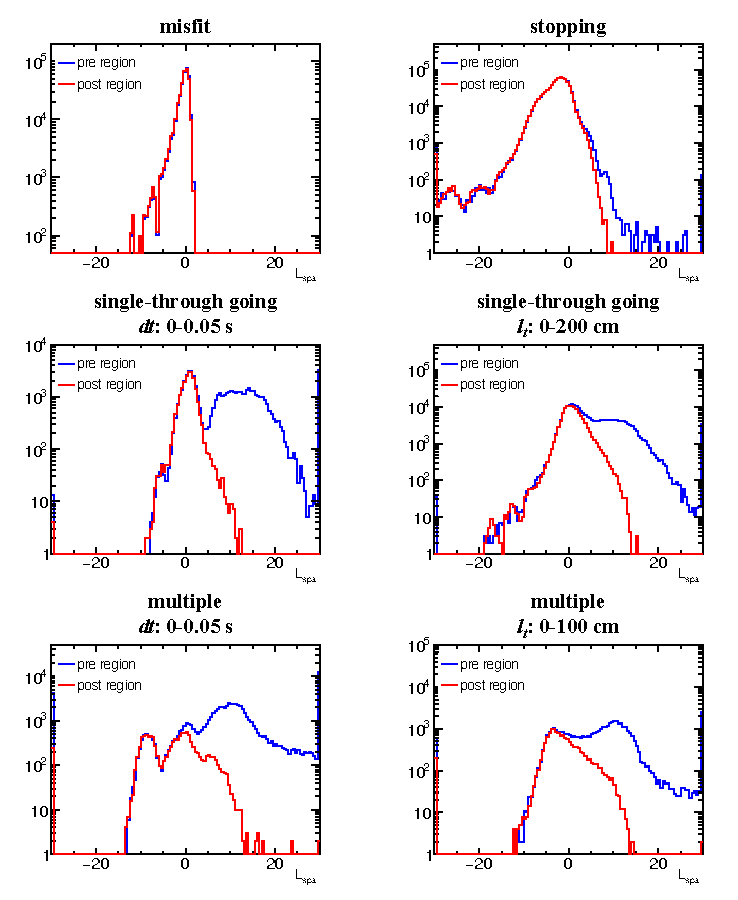
\includegraphics[width=16cm]{Figures/Selection/L_spall}
	\caption[$\mathcal{L}_{\rm spall}$ distributions ($E_{\rm vis}$: 7.49--9.49~MeV)]{
	$\mathcal{L}_{\rm spall}$ distributions ($E_{\rm vis}$: 7.49--9.49~MeV)~\cite{2023HaradaPhD}.
	Blue lines show muons in pre-region (time region from $-$60~s to 0~s with the SHE-triggered event as 0~s).
	Red lines show muons in post-region (time region from 0~s to 60~s with the SHE-triggered event as 0~s).
	}\label{L_spall}
\end{figure}

\clearpage

\subsubsection{Spallation box cut}\label{Sec_box}
\vs\hs
When $E_{\rm vis}$ exceeds 15.49~MeV, it is difficult to accurately optimize the spallation likelihood cut criteria because of the small statistics of muon spallation sample.
Therefore, the cut criteria summarized in Table~\ref{tab:box} are applied to SHE-triggered events primarily above 15.49~MeV.
In Table~\ref{tab:box}, $g_{\mu}$ is the muon reconstruction goodness.
Details of the muon event reconstruction are summarized in Ref.~\cite{2023HaradaPhD}.

\begin{table}[H]
	\centering
	\caption[Cut criteria of spallation box cut]{
	Cut criteria of spallation box cut~\cite{2023HaradaPhD}.
	}\label{tab:box}
	\vs
	\begin{tabular}{ccc} \hline \hline
		$E_{\rm vis}$ & Muon type & Cut criteria                                                         \\
		(MeV)         &           &                                                                      \\ \hline
		7.49--23.49   & -         & $dt < 0.1\,{\rm s}$ and $l_{t} < 400\,{\rm cm}$                      \\
		15.49--19.49  & misfit    & $dt < 1.5\,{\rm s}$                                                  \\
		15.49--17.49  & single    & $g_{\mu} \geq 0.4$ and $dt < 7\,{\rm s}$ and $l_{t} < 150\,{\rm cm}$ \\
		15.49--17.49  & stopping  & $g_{\mu} < 0.3$ and $dt < 6\,{\rm s}$                                \\
		15.49--19.49  & stopping  & $dt < 0.05\,{\rm s}$                                                 \\
		15.49--19.49  & multiple  & $dt < 0.05\,{\rm s}$                                                 \\ \hline \hline
	\end{tabular}
\end{table}

\subsubsection{Spallation cut efficiency}
\vs\hs
The expected number of events except for spallation events is scaled by using the spallation cut efficiency for random events $\varepsilon_{\rm random}$, which is equivalent to the signal efficiency after the spallation cut.
Moreover, the expected number of spallation events is scaled by using the spallation cut efficiency for $^{9}{\rm Li}$ events $\varepsilon_{\rm ^{9}Li}$.
Table~\ref{tab:spa} shows the spallation cut efficiency for random and $^{9}{\rm Li}$ events.
Details about how to estimate these efficiencies are summarized in Ref.~\cite{2023HaradaPhD}.

\begin{table}[H]
	\centering
	\caption[Spallation cut efficiency for random and $^{9}{\rm Li}$ events]{
	Spallation cut efficiency for random and $^{9}{\rm Li}$ events.
	}\label{tab:spa}
	\vs
	\begin{tabular}{ccc} \hline \hline
		$E_{\rm vis}$ & $\varepsilon_{\rm random}$ & $\varepsilon_{\rm ^{9}Li}$ \\
		(MeV)         &                            &                            \\ \hline
		7.49--9.49    & 51.8\%                     & 3.4\%                      \\
		9.49--11.49   & 78.2\%                     & 5.0\%                      \\
		11.49--13.49  & 86.0\%                     & 5.9\%                      \\
		13.49--15.49  & 93.1\%                     & 5.5\%                      \\
		15.49--17.49  & 73.4\%                     & 0.0\%                      \\
		17.49--19.49  & 81.8\%                     & 0.0\%                      \\
		19.49--23.49  & 86.1\%                     & 0.0\%                      \\
		23.49--29.49  & 96.1\%                     & 0.0\%                      \\ \hline \hline
	\end{tabular}
\end{table}





\subsection{Third reduction}
\subsubsection{Effective wall distance cut}
\vs\hs
Remaining radioactive backgrounds around the detector wall are removed using the effective wall distance ($d_{\rm eff}$).
The definition of $d_{\rm eff}$ is shown in Figure~\ref{effwall}, and the following cut criteria are applied to candidate events.
\begin{eqnarray}
	d_{\rm eff} < \left
	\{\begin{array}{lll}
		500\,{\rm cm}                                   & (7.49\,{\rm MeV} < E_{\rm vis} < 15.49\,{\rm MeV})  \\
		500 - 50 \times (E_{\rm vis} - 15.49)\,{\rm cm} & (15.49\,{\rm MeV} < E_{\rm vis} < 19.49\,{\rm MeV}) \\
		300\,{\rm cm}                                   & (19.49\,{\rm MeV} < E_{\rm vis} < 29.49\,{\rm MeV})
	\end{array}
	\right.
\end{eqnarray}
$d_{\rm eff}$ distributions are shown in Figure~\ref{Data_effwall}, Figure~\ref{ATM_effwall}, and Figure~\ref{Nuebar_effwall}.

\begin{figure}[h]
	\centering
	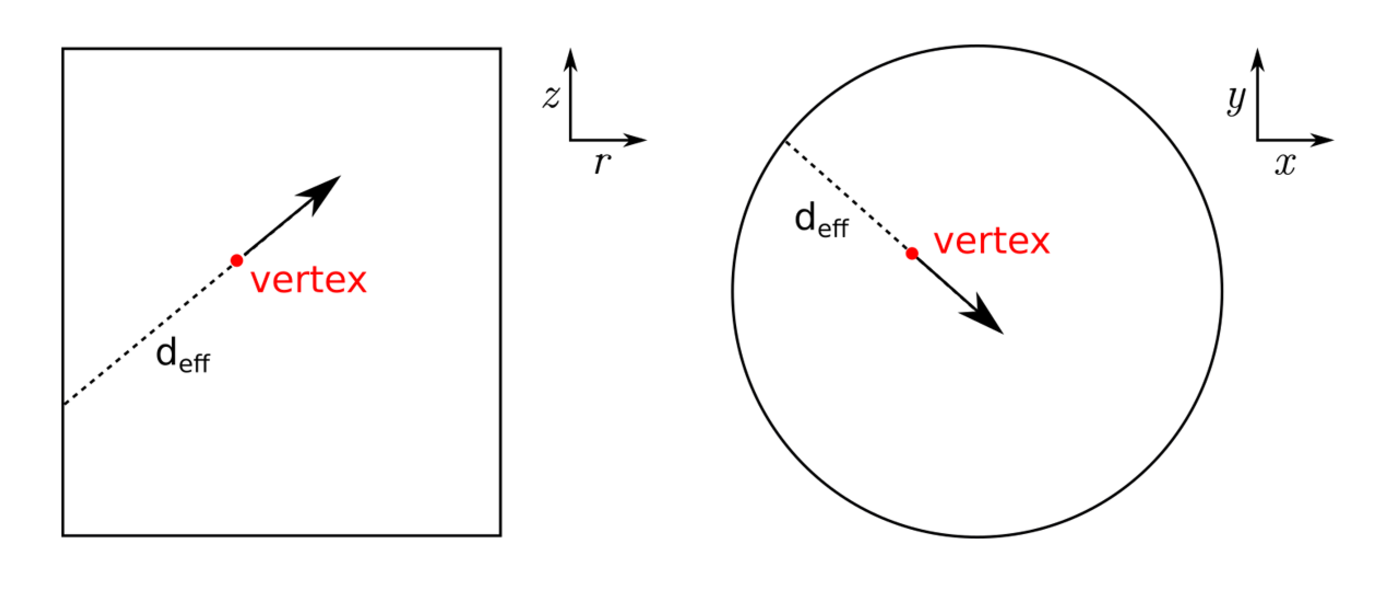
\includegraphics[width=10cm]{Figures/Selection/effwall}
	\caption[Definition of $d_{\rm eff}$]{
	Definition of $d_{\rm eff}$~\cite{2021Abe}.
	}\label{effwall}
\end{figure}

\subsubsection{Pre-activity cut and post-actvity cut}
\vs\hs
As shown in Figure~\ref{Selection_CC_numu_visible_CC_numu_02}, when a visible muon decays into an electron, or when de-excitation gamma-rays and an invisible muon are generated, the event may have two hit peaks within the time window of [$-$5, 35]~$\mu$s.
These events are removed by using the information of hit peaks before or after the main hit peak.
To remove events with hit peaks before the main hit peak, the TOF-subtracted time window of [$-$5~$\mu$s, $-$12~ns] from the main peak is scanned using a TOF-subtracted 15~ns time window to search the hit clusters.
When the maximal number of hits in a TOF-subtracted 15~ns time window is greater than 11, the event is removed.
Moreover, to remove events with hit peaks after the main hit peak, the number of decay electrons within 35~$\mu$s from the main hit peak ($N_{\rm decay\mathchar`-e}$) is searched using an algorithm used in previous SK analyses~\cite{2017Abe}.
When $N_{\rm decay\mathchar`-e}$ is greater or equal to 1, the event is removed.
$N_{\rm decay\mathchar`-e}$ distributions are shown in Figure~\ref{Data_nmue}, Figure~\ref{ATM_nmue}, and Figure~\ref{Nuebar_nmue}.

\begin{figure}[h]
	\centering
	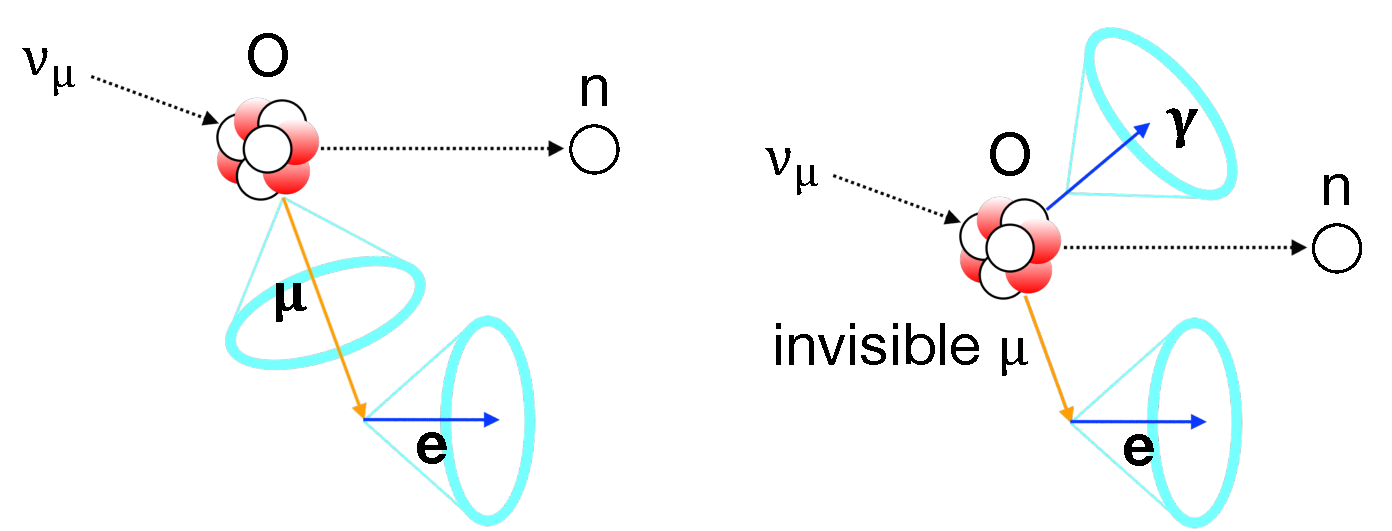
\includegraphics[width=12cm]{Figures/Selection/CC_numu_visible_CC_numu_02}
	\caption[Schematic view of atmospheric neutrino events with two hit peaks]{
	Schematic view of atmospheric neutrino events with two hit peaks.
	}\label{Selection_CC_numu_visible_CC_numu_02}
\end{figure}

\subsubsection{Ring cleanliness cut}\label{Sec_ring}
\vs\hs
Cherenkov rings caused by electrons and gamma-rays become fuzzy due to the electromagnetic shower, while Cherenkov rings caused by muons and pions become clear.
Events with visible muons and pions are removed by using the ring cleanliness ($L_{\rm cle}$).\\
\hs
Here, the calculation method of $L_{\rm cle}$ is described.
To calculate the $L_{\rm cle}$, PMT hits of the main hit peak in a TOF-subtracted 15~ns time window are used.
Given a reconstructed vertex, a combination of three hits uniquely determines a cone and the opening angle $\theta$.
In Figure~\ref{opening_angle},
\begin{eqnarray}
	\sin\theta &=& R \nonumber \\
	    \theta &=& \sin^{-1}R, \label{Eq_theta}
\end{eqnarray}
and from the law of sines,
\begin{eqnarray}
	{a \over \sin{A}} &=& 2R \nonumber \\
	                R &=& {a \over 2\sin{A}} \nonumber \\
	                  &=& {a \over 2\sqrt{1 - \cos^{2}A}} \nonumber \\
	                  &=& {a \over 2\sqrt{1 - {2b^{2}c^{2} - 2a^{2}b^{2} - 2c^{2}a^{2} + a^{4} + b^{4} + c^{4} \over 4b^{2}c^{2}}}}\,\,\Biggl(\because\,\,\cos{A} = {b^{2} + c^{2} - a^{2} \over 2bc}\Biggr) \nonumber \\
	                  &=& {abc \over \sqrt{4b^{2}c^{2} - (2b^{2}c^{2} - 2a^{2}b^{2} - 2c^{2}a^{2} + a^{4} + b^{4} + c^{4})}} \nonumber \\
	                  &=& {abc \over \sqrt{2(a^{2}b^{2} + b^{2}c^{2} + c^{2}a^{2}) - (a^{4} + b^{4} + c^{4})}}. \label{Eq_R}
\end{eqnarray}
Therefore, from Equation~(\ref{Eq_theta}) and Equation~(\ref{Eq_R}), $\theta$ is
\begin{eqnarray}
	\theta = \sin^{-1}\Biggl\{{abc \over \sqrt{2(a^{2}b^{2} + b^{2}c^{2} + c^{2}a^{2}) - (a^{4} + b^{4} + c^{4})}}\Biggr\}.
\end{eqnarray}
Then, $\theta$ for all combinations are filled in a histogram to determine the bin with most entries (${\rm bin}_{\rm most}$).
One example of the histogram of $\theta$ for all three hits combinations and the hit map is shown in Figure~\ref{L_cle}.
Finally, $L_{\rm cle}$ is calculated as
\begin{eqnarray}
	L_{\rm cle} = {N_{5\,{\rm bins}} \over N_{19\,{\rm bins}}},
\end{eqnarray}
where $N_{5\,{\rm bins}}$ ($N_{19\,{\rm bins}}$) shows the number of entries in five (nineteen) adjacent bins centered on ${\rm bin}_{\rm most}$.
In Figure~\ref{L_cle}, filled region (dotted line region) shows the five (nineteen) adjacent bins centered on ${\rm bin}_{\rm most}$.\\
\hs
Events with visible muons and pions tend to have the large $L_{\rm cle}$.
In this study, events that $L_{\rm cle}$ is greater than 0.36 are removed.
$L_{\rm cle}$ distributions are shown in Figure~\ref{Data_pilike}, Figure~\ref{ATM_pilike}, and Figure~\ref{Nuebar_pilike}.

\begin{figure}[p]
	\centering
	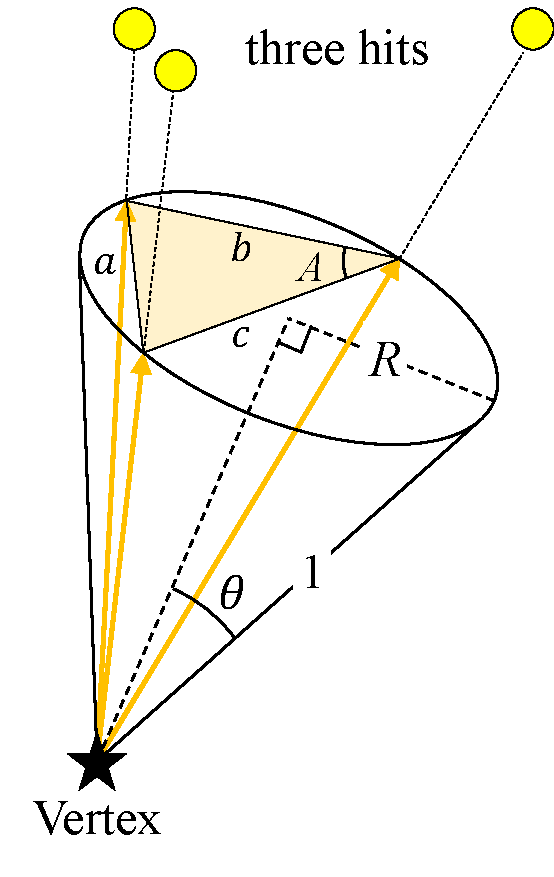
\includegraphics[width=6cm]{Figures/Selection/opening_angle}
	\caption[Definition of $\theta$]{
	Definition of $\theta$.
	}\label{opening_angle}
\end{figure}

\begin{figure}[p]
	\centering
	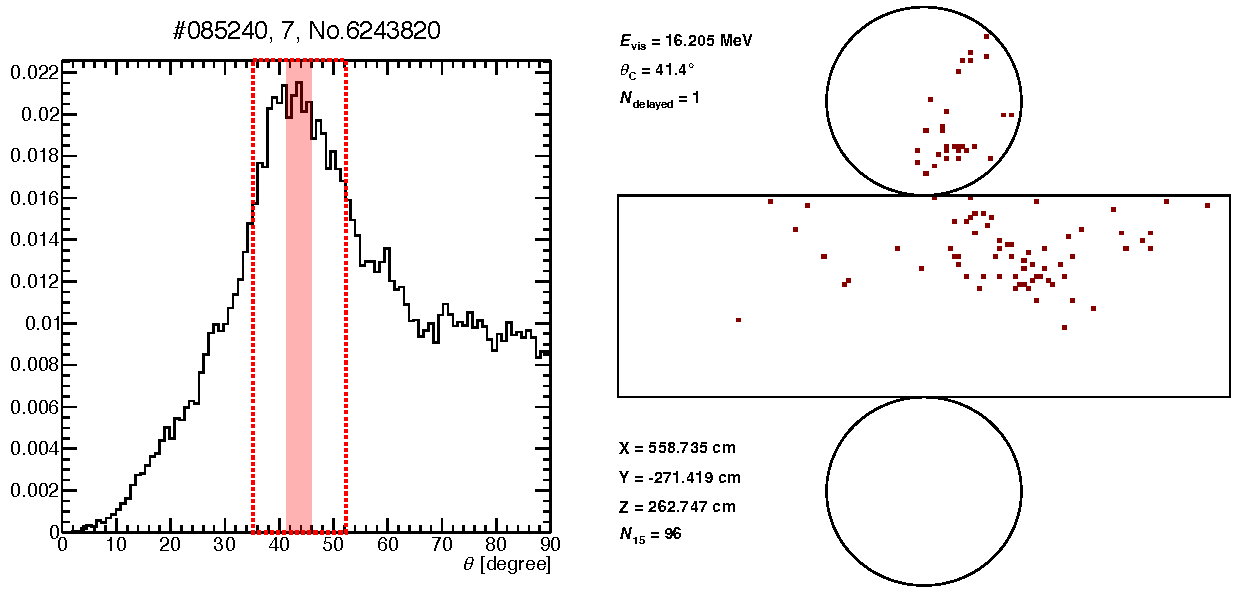
\includegraphics[width=16cm]{Figures/Selection/L_cle}
	\caption[Histogram of $\theta$ for all three hits combinations and the hit map]{
	Histogram of $\theta$ for all three hits combinations (left) and the hit map (right).
	In the histogram, filled region (dotted line region) shows the five (nineteen) adjacent bins centered on the bin with most entries (${\rm bin}_{\rm most}$).
	In the right figure, top circle, center rectangle, and bottom circle show the SK top, barrel, and bottom, respectively.
	$\theta_{{\rm C}}$ is the reconstructed Cherenkov angle of the prompt signal (described in Section~\ref{Sec_theta_delayed}), $N_{\rm delayed}$ is the number of delayed signals per event (described in Section~\ref{Sec_theta_delayed}), X, Y, and Z are the reconstructed vertices, and $N_{15}$ is the number of hits in a TOF-subtracted 15~ns time window.
	In this case, the total number of entries in the histogram is ${}_{N_{15}}{\rm C}_{3} = {}_{96}{\rm C}_{3} = 142{,}880$.
	Note that this histogram is normalized.
	}\label{L_cle}
\end{figure}

\subsubsection{Charge over hit cut}
\vs\hs
As described in Section~\ref{Sec_ring}, Cherenkov rings caused by muons and pions become clear, and more charge is deposited on a single PMT compared to electrons.
Events with visible muons and pions are further removed by using the ratio of charge to the number of hits in a TOF-subtracted 50~ns time window centered on the main hit peak ($Q_{50}/N_{50}$).
Events with visible muons and pions tend to have the large $Q_{50}/N_{50}$.
In this study, events that $Q_{50}/N_{50}$ is greater than 2 are removed.
$Q_{50}/N_{50}$ distributions are shown in Figure~\ref{Data_q50n50}, Figure~\ref{ATM_q50n50}, and Figure~\ref{Nuebar_q50n50}.





\subsection{Cherenkov angle cut and neutron tagging}\label{Sec_theta_delayed}
\vs\hs
Finally, we select NCQE events using the reconstructed Cherenkov angle of the prompt signal ($\theta_{{\rm C}}$) and the number of delayed signals per event ($N_{{\rm delayed}}$).

\subsubsection{Reconstructed Cherenkov angle of the prompt signal}
\vs\hs
$\theta_{{\rm C}}$ is calculated using the histogram of $\theta$ for all three hits combinations described in Section~\ref{Sec_ring}.
In the histogram, the seven adjacent bins with most entries are determined, and the upper border of the center bin is taken as $\theta_{\rm C}$ (see Figure~\ref{theta_C}).

\begin{figure}[h]
	\centering
%	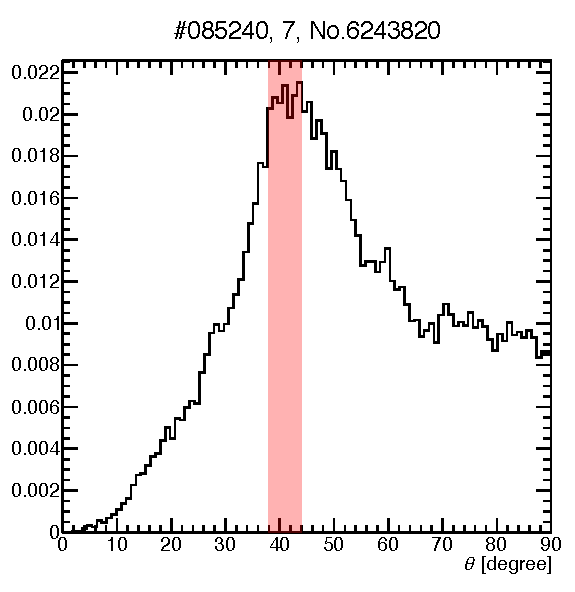
\includegraphics[width=6cm]{Figures/Selection/theta_C}
	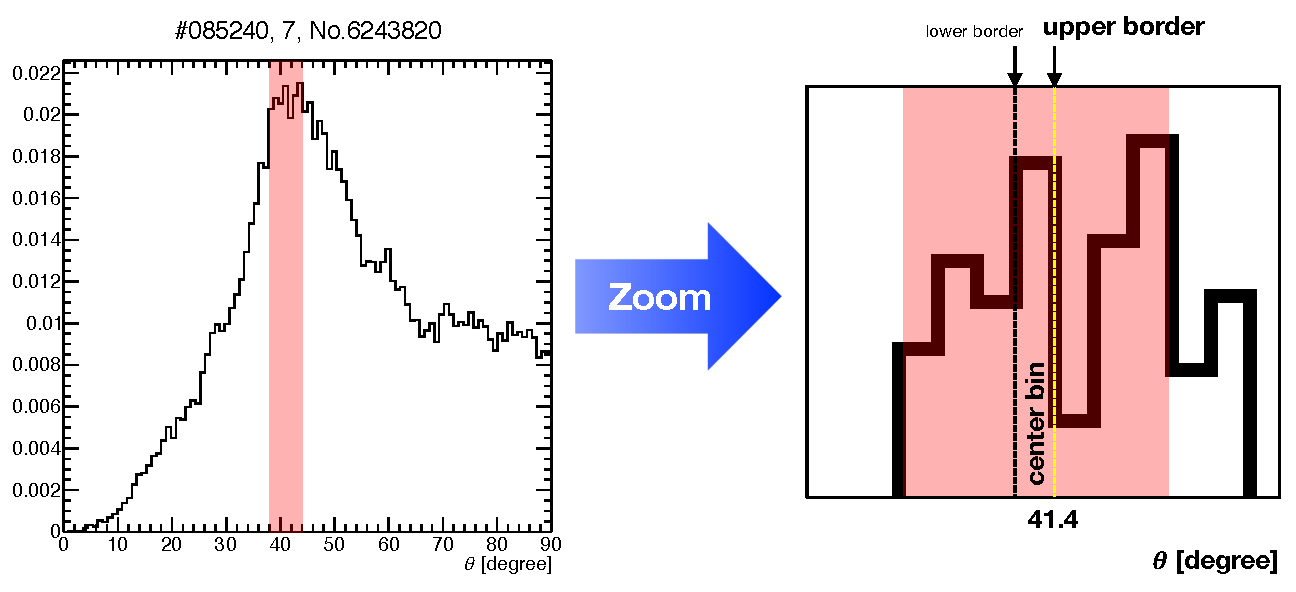
\includegraphics[width=12cm]{Figures/Selection/theta_C_03}
	\caption[Histogram of $\theta$ for all three hits combinations]{
	Histogram of $\theta$ for all three hits combinations.
	This histogram is the same as the histogram shown in Figure~\ref{L_cle}.
	Filled region shows the seven adjacent bins with most entries, and in this case $\theta_{\rm C}$ is taken to be 41.4~degrees.
	}\label{theta_C}
\end{figure}

\subsubsection{Number of delayed signals per event}\label{Subsubsec_Ndelayed}
\vs\hs
Here, the neutron tagging method is explained.
Figure~\ref{Selection_neutron_tagging} shows the schematic view of neutron candidate search.
First, neutron candidates are searched by 25 PMT hits/200~ns trigger in the region of [4, 535]~$\mu$s from the prompt signal.
Then all neutron candidates are reconstructed, and delayed signals from neutron capture on Gd are selected based on the following selection criteria.
\begin{itemize}
%	\item $N_{200} \geq 25$
	\item Distance from the ID wall is larger than 2~m
	\item Timing is after 4~$\mu$s from the prompt signal
	\item $g_{\rm vtx} > 0.4$ and $g_{\rm dir} < 0.4$
	\item $E_{\rm vis} > 2.99\,{\rm MeV}$
	\item Distance from the prompt vertex is smaller than 3~m
\end{itemize}
$N_{{\rm delayed}}$ is the number of delayed signals that satisfy the above selection criteria.

\begin{figure}[H]
	\centering
	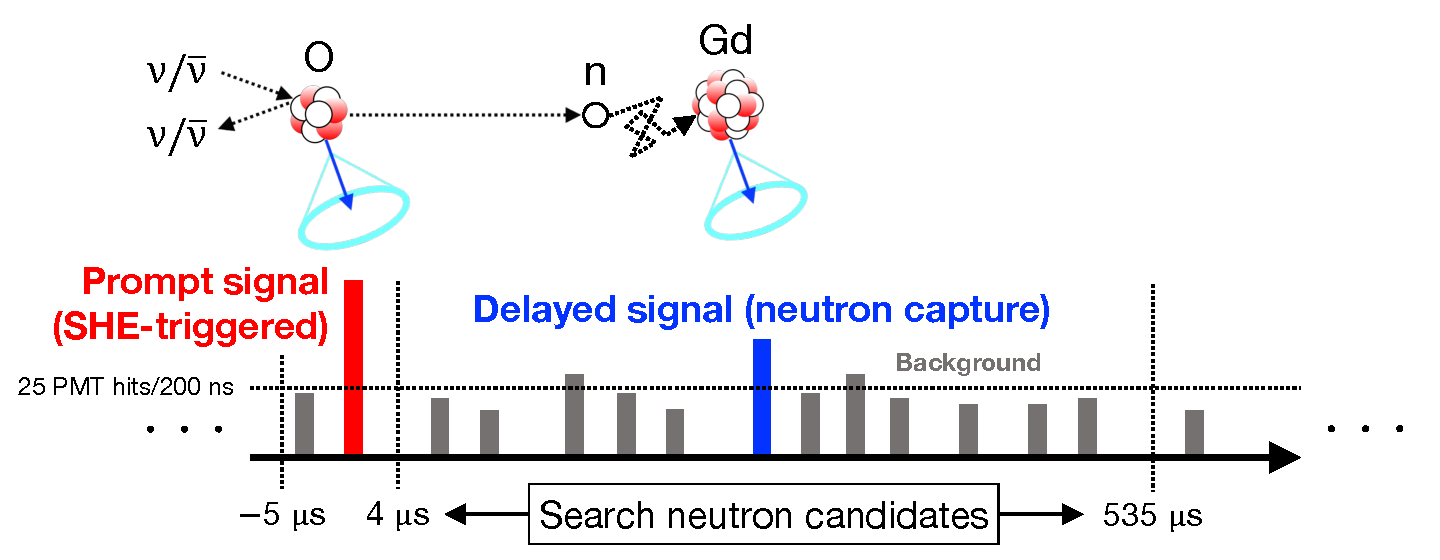
\includegraphics[width=16cm]{Figures/Selection/neutron_tagging}
	\caption[Schematic view of neutron candidate search]{
	Schematic view of neutron candidate search.
	}\label{Selection_neutron_tagging}
\end{figure}

\subsubsection{Difference between this study and the DSNB search in SK-VI}
\vs\hs
The difference between this study and the DSNB search in SK-VI~\cite{2023Harada} is the cut criteria of $\theta_{{\rm C}}$ and $N_{{\rm delayed}}$.
In IBD events, only one relativistic positron and one neutron are emitted (see Figure~\ref{DSNB_NCQE}).
Therefore, $\theta_{{\rm C}}$ and $N_{{\rm delayed}}$ tend to be about 42~degrees and one, respectively.
While, in an NCQE event, multiple gamma-rays and multiple neutrons are easily emitted (see Figure~\ref{Introd_NCQE_PriSec}).
When multiple gamma-rays are emitted, $\theta_{{\rm C}}$ tends to be larger because of the uniform distribution of the hit PMTs.
Therefore, in this study, we select the events that $\theta_{{\rm C}}$ is greater than 50~degrees and $N_{{\rm delayed}}$ is greater or equal to one.
The cut criteria of $\theta_{{\rm C}}$ and $N_{{\rm delayed}}$ are the same as the study in SK pure water phase~\cite{2019Linyan}.
$\theta_{\rm C}$ distributions are shown in Figure~\ref{Data_angle}, Figure~\ref{ATM_angle}, and Figure~\ref{Nuebar_angle}.
Moreover, $N_{\rm delayed}$ distributions are shown in Figure~\ref{Data_RecoNumCap}, Figure~\ref{ATM_RecoNumCap}, and Figure~\ref{Nuebar_RecoNumCap}.





\subsection{Observed and expected number of events}
\vs\hs
After applying all event selections to 552.2~days of SK-VI data, 38~events remain.
Figure~\ref{Figure07} shows the vertex distribution of prompt signals and delayed signals for the data.
From this figure, we confirmed that these events are uniformly distributed.\\
\hs
The expected number of events in each secondary interaction model estimated by the simulation are summarized in Table~\ref{tab:num}.
After applying all event selections, NCQE and NC non-QE events account for about 60\% and about 30\% of total events, respectively.
Note that the number of DSNB events predicted by the Horiuchi~$+$~09 model~\cite{2009Horiuchi}, which is not used in this study, is 0.0854.
Moreover, the number of atmospheric neutrino events is larger in BERT than other two models.
The difference of the number of atmospheric neutrino events comes from the number of de-excitation gamma-rays and neutrons by secondary interactions (see Section~\ref{Sec_Model}).\\
\hs
Figure~\ref{FTFP_BERT_HP_Figure02_Poisson}, Figure~\ref{FTFP_BERT_HP_Figure08_Poisson}, and Figure~\ref{FTFP_BERT_HP_Figure04_Poisson} show the distributions of $\theta_{\rm C}$, $E_{\rm vis}$, and $N_{\rm delayed}$ in BERT, respectively.
From these figures, we can see that the tendency of distribution is similar between NCQE and NC non-QE events.
\\
\hs
The NCQE cumulative signal efficiencies as a function of $E_{\rm vis}$ are shown in Figure~\ref{BERT_Figure05}.
Moreover, the NCQE cumulative signal efficiencies at each event reduction are summarized in Table~\ref{tab:eff}.
Signal efficiencies of $\theta_{\rm C}$ cut and $N_{\rm delayed}$ cut increase as $E_{\rm vis}$ increases.
This means that $E_{\rm vis}$ is correlated to the number of de-excitation gamma-rays and neutrons by secondary interactions.
Other distributions related to this section are summarized in Appendix~\ref{App_Selection}.

\begin{figure}[h]
	\centering
	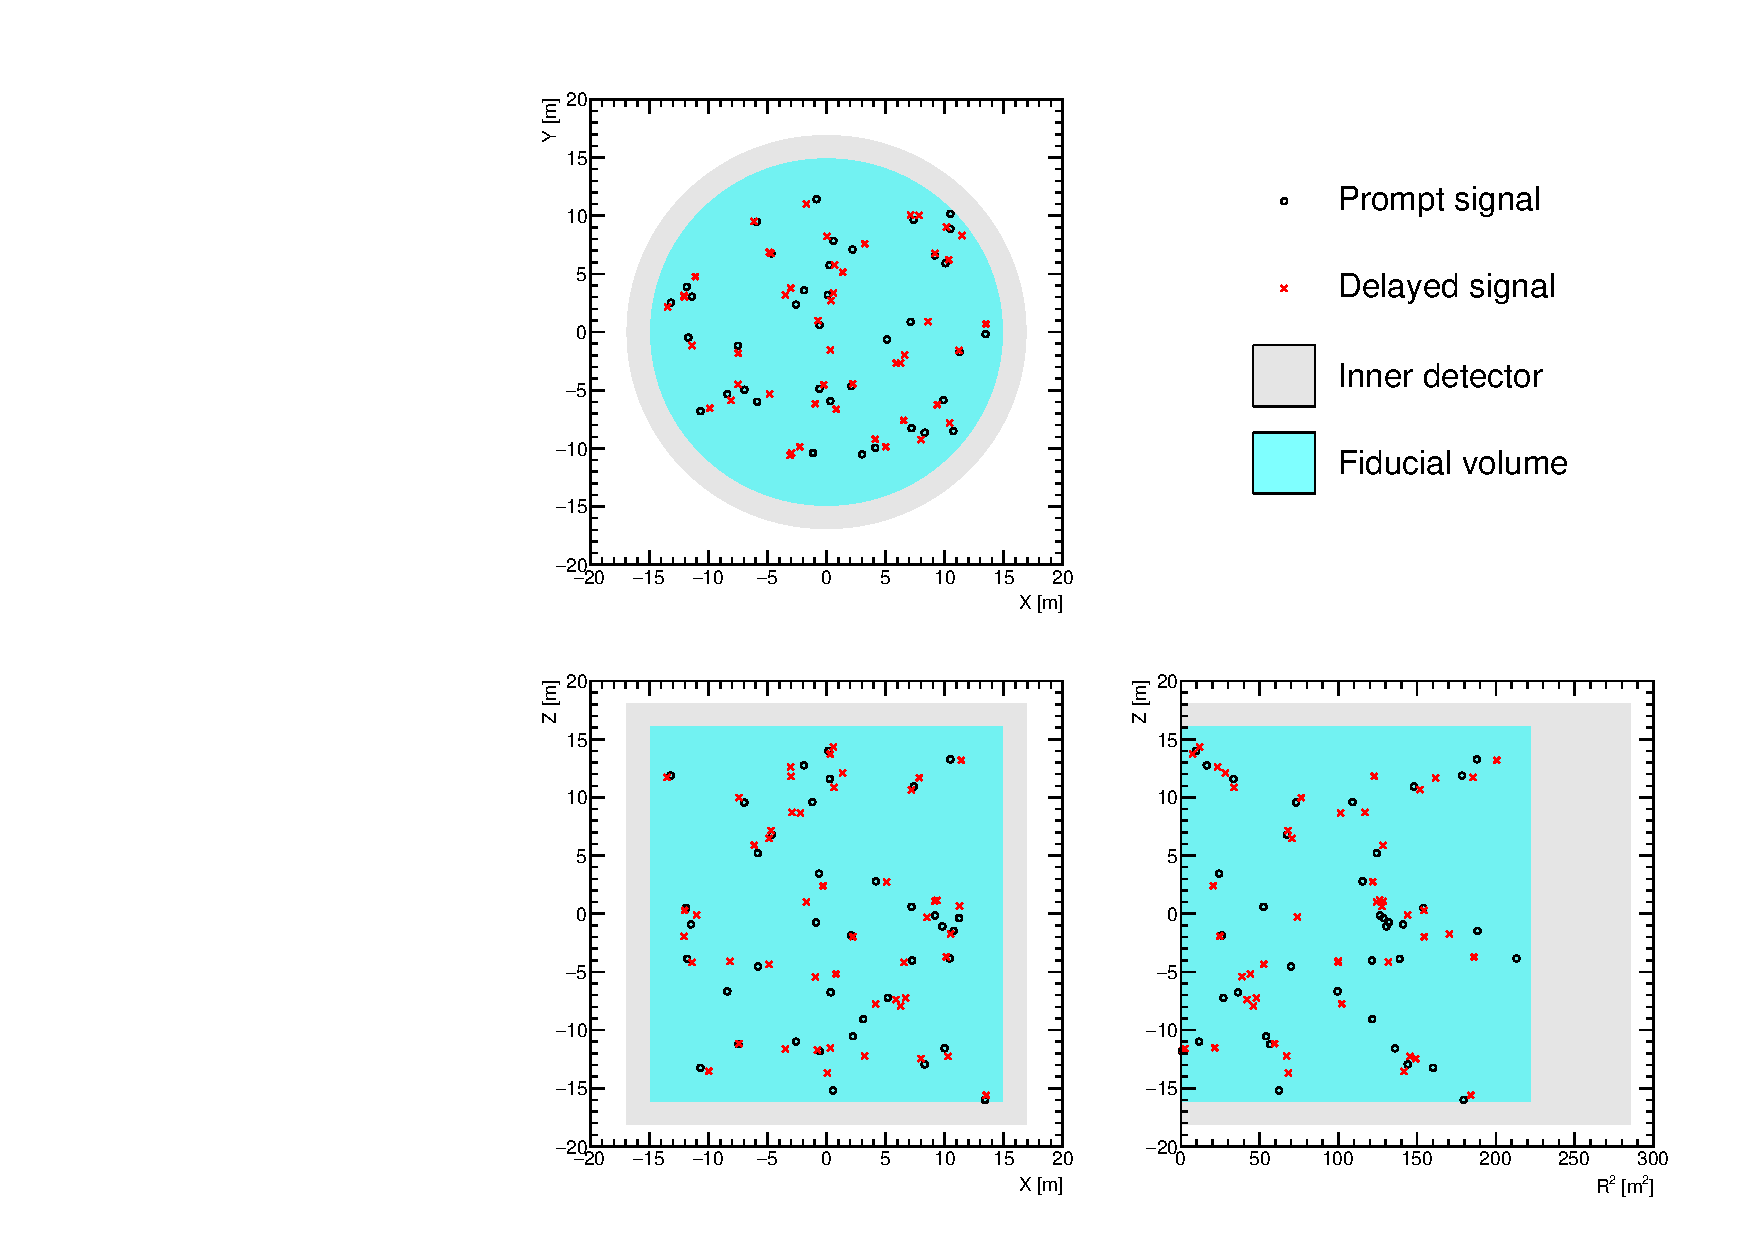
\includegraphics[width=14cm]{PDF/Figure07/Figure07_prompt_delay}
	\caption[Vertex distribution of prompt signals and delayed signals for the data]{
	Vertex distribution of prompt signals and delayed signals for the data.
	}\label{Figure07}
\end{figure}

\begin{table}[h]
	\centering
	\caption[The expected number of events in each secondary interaction model]{
	The expected number of events in each secondary interaction model.
	The fractions are summarized in parentheses.
	The expected number of spallation, reactor neutrino, and accidental coincidence events, which are calculated by the same method as Ref.~\cite{2023Harada}, are common to each model.
	}\label{tab:num}
	\vs
	\begin{tabular}{lccc} \hline \hline
		                       & BERT             & BIC              & INCL++           \\ \hline
		Total                  & 45.8991          & 33.6573          & 33.9739          \\ \hline
		NCQE                   & 28.7071 (62.5\%) & 19.8420 (59.0\%) & 20.2027 (59.5\%) \\
		NC non-QE              & 13.2721 (28.9\%) & 10.1887 (30.3\%) & 10.0517 (29.6\%) \\
		CC                     & 1.4177 (3.1\%)   & 1.1244 (3.3\%)   & 1.2173 (3.6\%)   \\ \hline
		Spallation             & 0.8879 (1.9\%)   & 0.8879 (2.6\%)   & 0.8879 (2.6\%)   \\
		Reactor neutrino       & 0.0619 (0.1\%)   & 0.0619 (0.2\%)   & 0.0619 (0.2\%)   \\
		Accidental coincidence & 1.5524 (3.4\%)   & 1.5524 (4.6\%)   & 1.5524 (4.6\%)   \\ \hline \hline
	\end{tabular}
\end{table}

\begin{figure}[h]
	\centering
	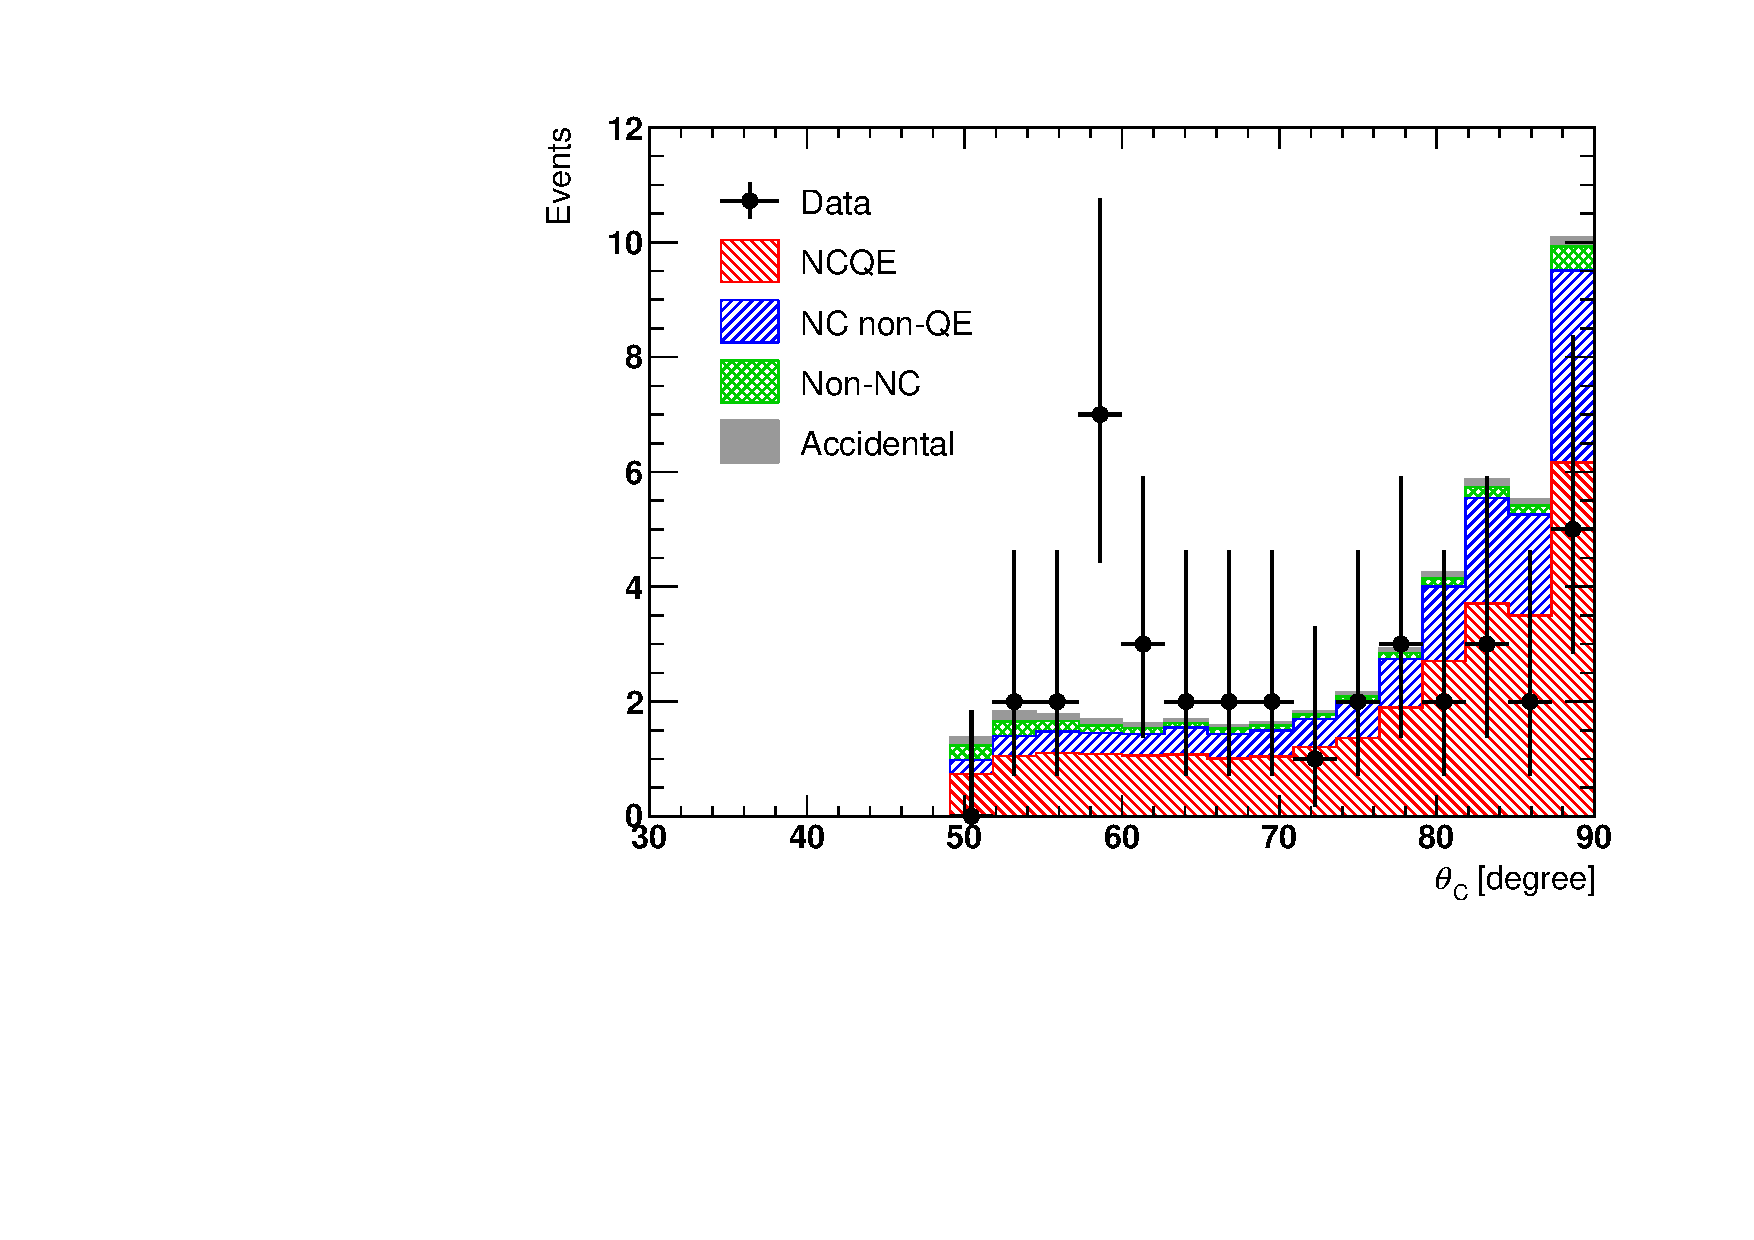
\includegraphics[width=12cm]{PDF/Figure02_02/FTFP_BERT_HP/Figure02_Poisson}
	\caption[$\theta_{\rm C}$ distribution in BERT]{
	$\theta_{\rm C}$ distribution in BERT.
	Non-NC includes CC, spallation, and reactor neutrino events.
	In this distribution, $E_{\rm vis}$ is between 7.49~MeV and 29.49~MeV and $N_{\rm delayed}$ is greater or equal to one.
	}\label{FTFP_BERT_HP_Figure02_Poisson}
\end{figure}

\begin{figure}[h]
	\centering
	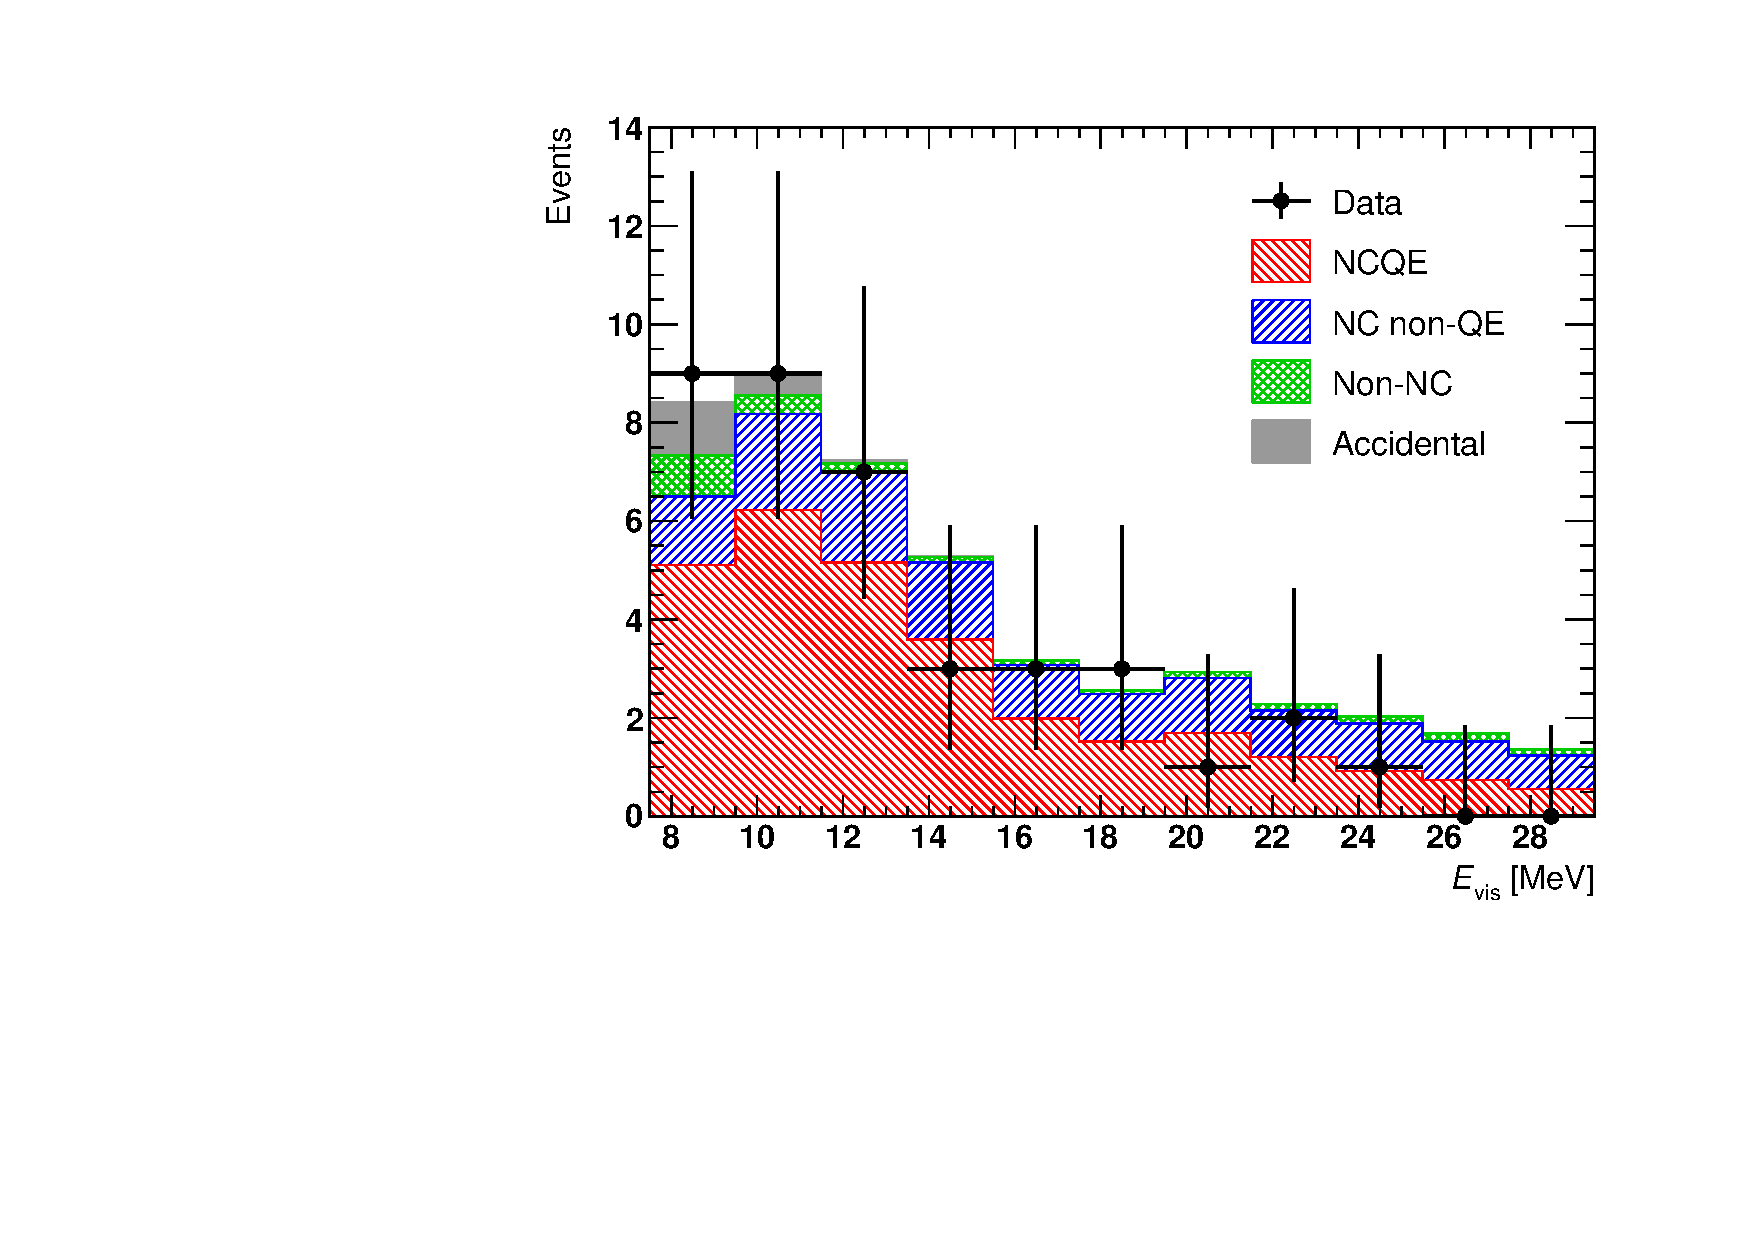
\includegraphics[width=12cm]{PDF/Figure08/FTFP_BERT_HP/Figure08_Poisson}
	\caption[$E_{\rm vis}$ distribution in BERT]{
	$E_{\rm vis}$ distribution in BERT.
	Non-NC includes CC, spallation, and reactor neutrino events.
	In this distribution, $\theta_{\rm C}$ is greater than 50~degrees and $N_{\rm delayed}$ is greater or equal to one.
	}\label{FTFP_BERT_HP_Figure08_Poisson}
\end{figure}

\begin{figure}[h]
	\centering
	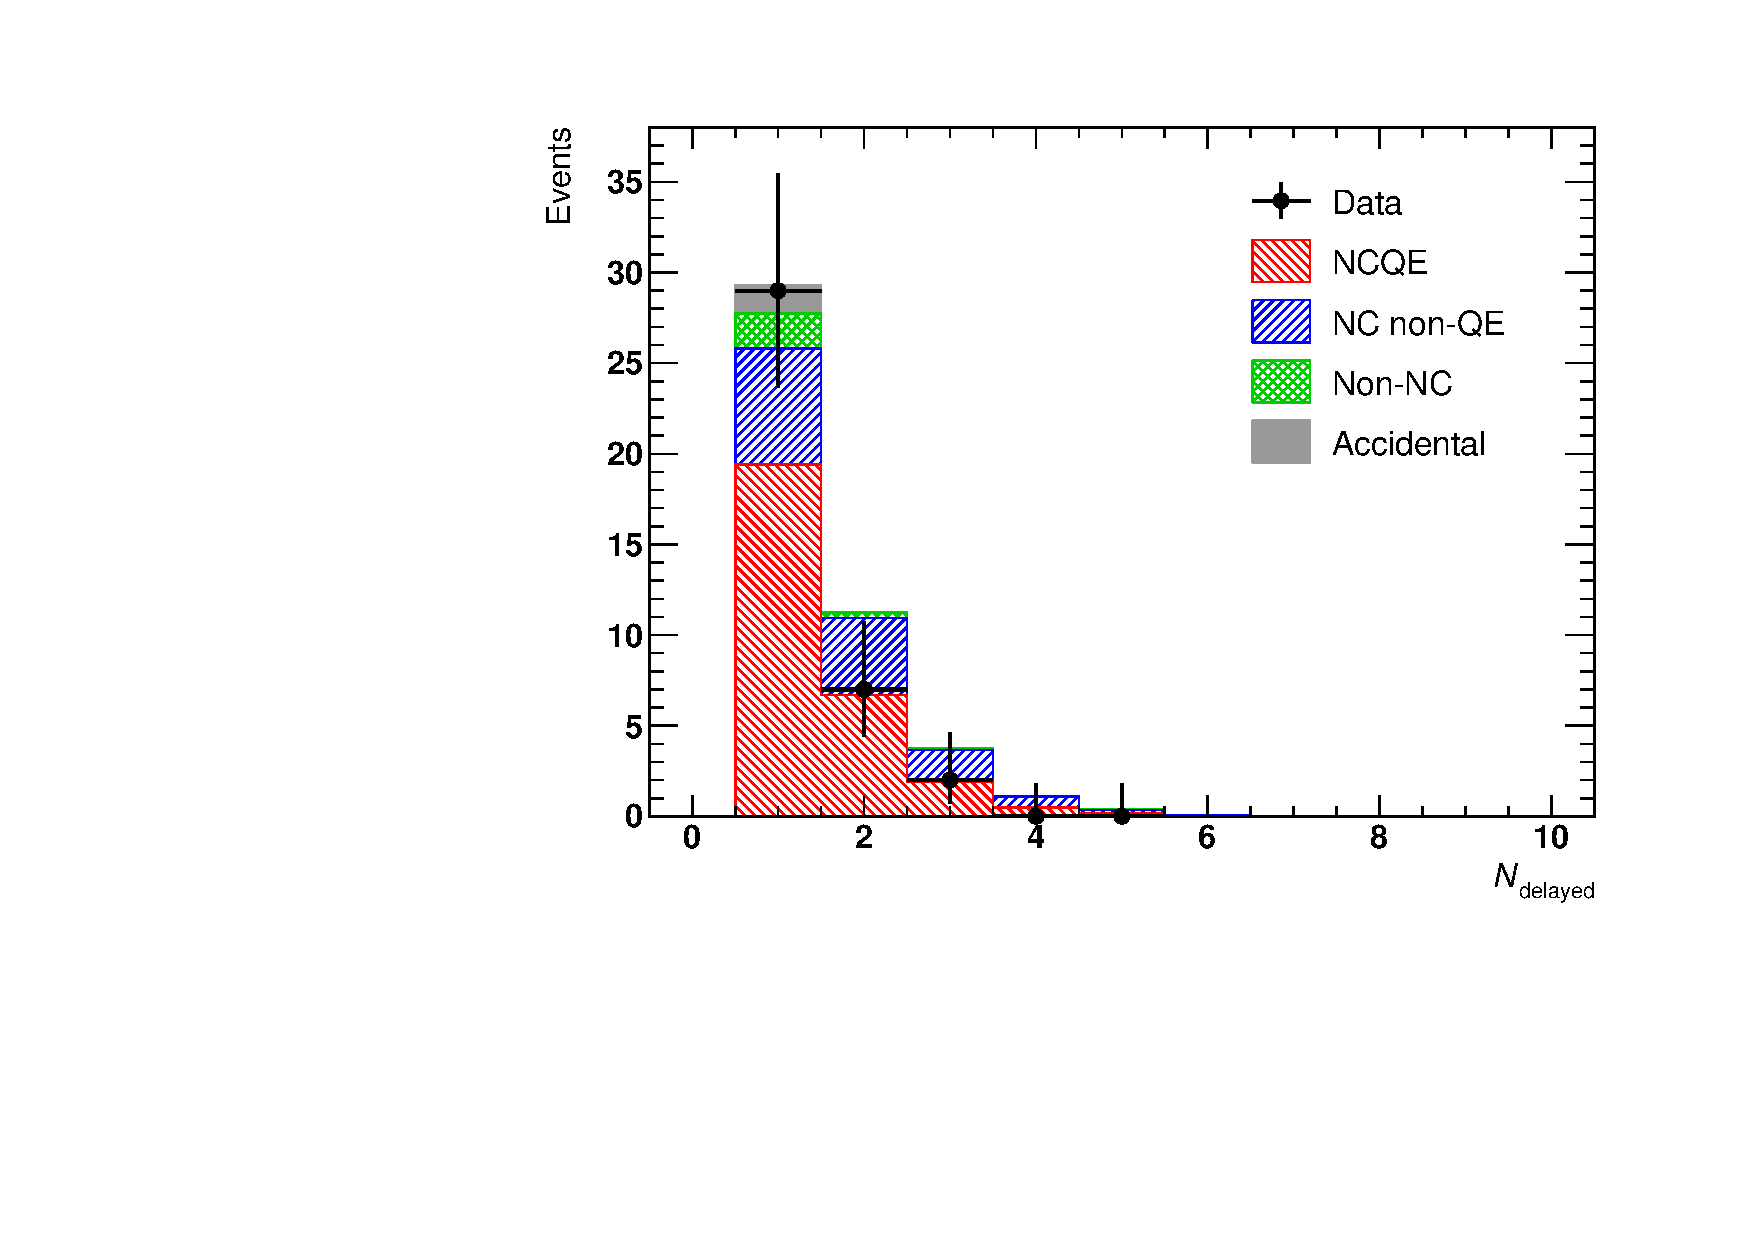
\includegraphics[width=12cm]{PDF/Figure04/FTFP_BERT_HP/Figure04_Poisson}
	\caption[$N_{\rm delayed}$ distribution in BERT]{
	$N_{\rm delayed}$ distribution in BERT.
	Non-NC includes CC, spallation, and reactor neutrino events.
	In this distribution, $\theta_{\rm C}$ is greater than 50~degrees and $E_{\rm vis}$ is between 7.49~MeV and 29.49~MeV.
	}\label{FTFP_BERT_HP_Figure04_Poisson}
\end{figure}

\begin{figure}[h]
	\centering
	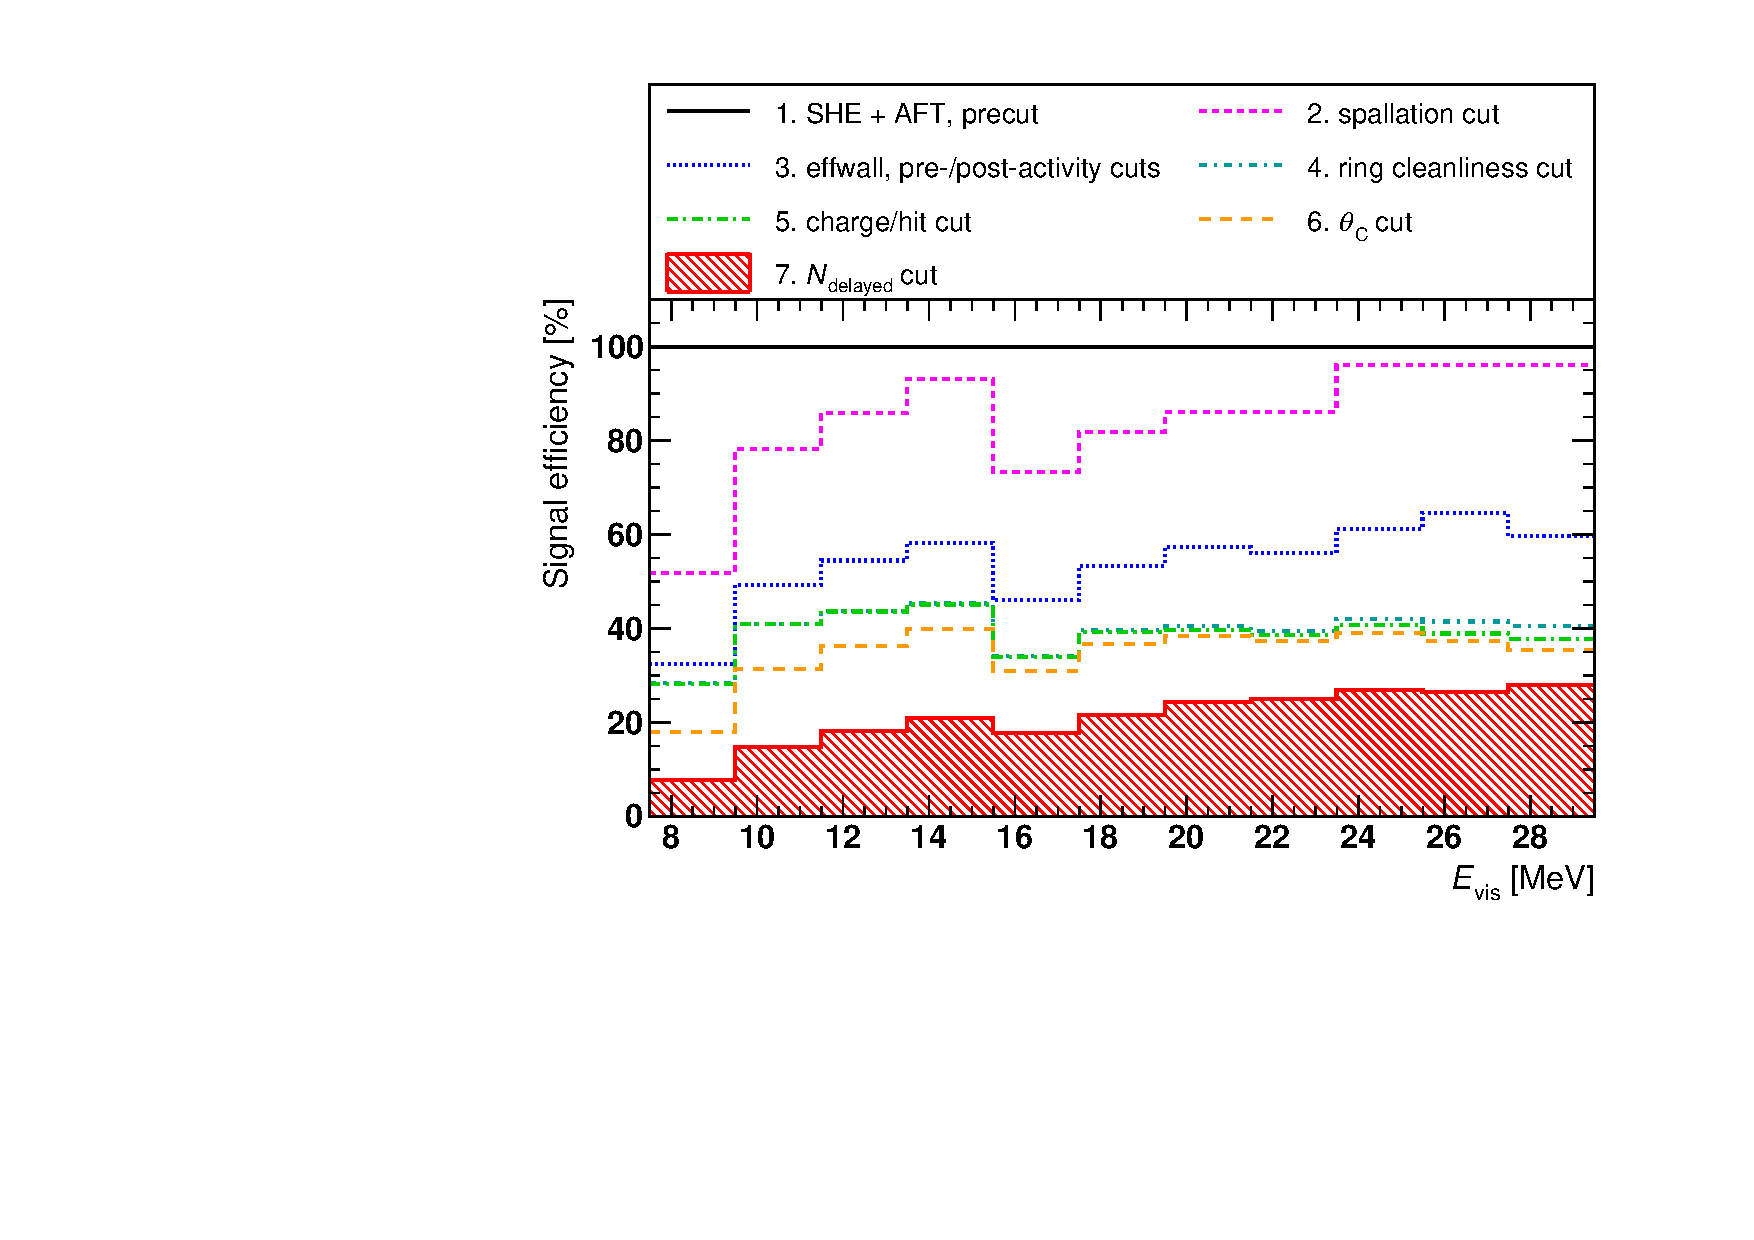
\includegraphics[width=12cm]{PDF/Figure05/FTFP_BERT_HP/Figure05}
	\caption[NCQE cumulative signal efficiencies as a function of $E_{\rm vis}$]{
	NCQE cumulative signal efficiencies as a function of $E_{\rm vis}$.
	Event reductions are performed in the order shown in the legend, and before the reduction for spallation events is taken as 100\%.
	}\label{BERT_Figure05}
\end{figure}

\begin{table}[h]
	\centering
	\caption[NCQE cumulative signal efficiencies at each event reduction]{
	NCQE cumulative signal efficiencies at each event reduction.
	}\label{tab:eff}
	\vs
	\begin{tabular}{lcccc} \hline \hline
		$E_{\rm vis}$ (MeV)   & 7.49--9.49   & 9.49--11.49  & 11.49--13.49 & 13.49--15.49 \\ \hline
		Spallation cut        & 51.8\%       & 78.2\%       & 86.0\%       & 93.1\%       \\
		$d_{\rm eff}$ cut     & 91.6\%       & 92.2\%       & 92.7\%       & 92.4\%       \\
		Pre-activity cut      & 99.5\%       & 99.4\%       & 99.2\%       & 98.6\%       \\
		Post-activity cut     & 68.8\%       & 68.8\%       & 68.9\%       & 68.7\%       \\
		$L_{\rm cle}$ cut     & 87.2\%       & 83.0\%       & 80.4\%       & 77.8\%       \\
		$Q_{50}/N_{50}$ cut   & 99.8\%       & 99.8\%       & 99.6\%       & 99.5\%       \\
		$\theta_{\rm C}$ cut  & 63.8\%       & 76.9\%       & 83.0\%       & 88.5\%       \\
		$N_{\rm delayed}$ cut & 42.5\%       & 46.8\%       & 50.5\%       & 52.6\%       \\ \hline
		All cuts              &  7.7\%       & 14.7\%       & 18.3\%       & 21.0\%       \\ \hline \hline
		                      &              &              &              &              \\ \hline \hline
		$E_{\rm vis}$ (MeV)   & 15.49--17.49 & 17.49--19.49 & 19.49--21.49 & 21.49--23.49 \\ \hline
		Spallation cut        & 73.4\%       & 81.8\%       & 86.1\%       & 86.1\%       \\
		$d_{\rm eff}$ cut     & 93.6\%       & 96.7\%       & 98.6\%       & 99.2\%       \\
		Pre-activity cut      & 98.0\%       & 97.2\%       & 96.7\%       & 95.6\%       \\
		Post-activity cut     & 68.3\%       & 69.3\%       & 69.9\%       & 68.7\%       \\
		$L_{\rm cle}$ cut     & 74.3\%       & 74.4\%       & 70.6\%       & 70.3\%       \\
		$Q_{50}/N_{50}$ cut   & 99.1\%       & 98.9\%       & 98.2\%       & 97.9\%       \\
		$\theta_{\rm C}$ cut  & 91.6\%       & 93.5\%       & 96.8\%       & 96.6\%       \\
		$N_{\rm delayed}$ cut & 57.4\%       & 58.9\%       & 63.4\%       & 67.1\%       \\ \hline
		All cuts              & 17.8\%       & 21.6\%       & 24.4\%       & 25.0\%       \\ \hline \hline
		                      &              &              &              &              \\ \hline \hline
		$E_{\rm vis}$ (MeV)   & 23.49--25.49 & 25.49--27.49 & 27.49--29.49 & 7.49--29.49  \\ \hline
		Spallation cut        & 96.1\%       & 96.1\%       & 96.1\%       & 72.6\%       \\
		$d_{\rm eff}$ cut     & 98.6\%       & 98.7\%       & 98.6\%       & 93.3\%       \\
		Pre-activity cut      & 94.8\%       & 95.1\%       & 91.9\%       & 98.6\%       \\
		Post-activity cut     & 68.1\%       & 71.5\%       & 68.6\%       & 68.9\%       \\
		$L_{\rm cle}$ cut     & 68.7\%       & 64.3\%       & 67.9\%       & 80.2\%       \\
		$Q_{50}/N_{50}$ cut   & 97.0\%       & 93.9\%       & 93.0\%       & 99.3\%       \\
		$\theta_{\rm C}$ cut  & 95.9\%       & 95.9\%       & 93.9\%       & 79.3\%       \\
		$N_{\rm delayed}$ cut & 69.0\%       & 70.9\%       & 79.1\%       & 51.3\%       \\ \hline
		All cuts              & 27.0\%       & 26.4\%       & 28.0\%       & 14.9\%       \\ \hline \hline
	\end{tabular}
\end{table}






\newpage

